\documentclass[9pt,twocolumn,twoside,lineno]{BioRxiv}
% Use the documentclass option 'lineno' to view line numbers
\setlength{\marginparwidth}{2cm}
\usepackage[textsize=tiny,colorinlistoftodos]{todonotes} % comments in margins
\definecolor{cornflowerblue}{rgb}{0.39, 0.58, 0.93}
\usepackage{blindtext}
\usepackage{gensymb}
\usepackage[switch]{lineno} 
\usepackage{pdfpages}

\def\code#1{\texttt{#1}}

%%%%%%%Add comments in color
\newcommand{\citex}[1]{{\small \textcolor{red}{CITE(#1)}}}
\newcommand{\X}{{\textcolor{red}{X}}}





\newcolumntype{b}{X}
\newcolumntype{s}{>{\hsize=.5\hsize}X}

% Set supplement numbers to S and start counting newly
\newcommand{\beginsupplement}{%
        \setcounter{table}{0}
        \renewcommand{\thetable}{S\arabic{table}}%
        \setcounter{figure}{0}
        \renewcommand{\thefigure}{S\arabic{figure}}%
     }


\title{Adaptive teosinte introgression modulates phospholipid levels and flowering time in maize}


\author[a,b,1]{Fausto Rodríguez-Zapata}
\author[a,1]{Allison C Barnes}
\author[b,1]{Karla A Blöcher-Juárez}
\author[c]{Dan Gates}
\author[a]{Andi Kur}
\author[d]{Li Wang}
\author[d]{Garrett M Janzen}
\author[e]{Sarah Jensen}
\author[b]{Juan M Estévez-Palmas}
\author[f]{Taylor Crow}
\author[b]{Rocío Aguilar-Rangel}
\author[g]{Edgar Demesa-Arevalo}
\author[g]{Tara Skopelitis}
\author[b]{Sergio Pérez-Limón}
\author[a, h]{Whitney L Stutts}
\author[h]{Yu-Chun Chiu}
\author[g]{David Jackson}
\author[i]{Oliver Fiehn}
\author[f]{Daniel Runcie}
\author[e]{Edward S Buckler}
\author[c]{Jeffrey Ross-Ibarra}
\author[d]{Matthew B. Hufford}
\author[b,j]{Ruairidh JH Sawers}
\author[a, b, *]{Rubén Rellán-Álvarez}

\affil[a]{Department of Molecular and Structural Biochemistry, North Carolina State University, Raleigh, NC}
\affil[b]{National Laboratory of Genomics for Biodiversity, Irapuato, México}
\affil[c]{Department of Evolution and Ecology, Center for Population Biology and Genome Center, University of California, Davis, CA}
\affil[e]{US Department of Agriculture–Agricultural Research Service, Cornell University, Ithaca, NY}
\affil[f]{Department of Plant Sciences, University of California, Davis, CA}
\affil[d]{Department of Ecology, Evolution, and Organismal Biology, Iowa State University, Ames, USA}
\affil[g]{Cold Spring Harbor Laboratory, Cold Spring Harbor, NY, USA}
\affil[h]{Molecular Education, Technology and Research Innovation Center, North Carolina State University, Raleigh, NC}
\affil[i]{West Coast Metabolomics Center, University of California, Davis, CA, USA}
\affil[j]{Department of Plant Science, The Pennsylvania State University, PA, USA}

\keywords{phospholipid metabolism; maize genetics; highland adaptation; convergent evolution}

\runningtitle{\textit{HPC1} selection in highland maize} % For use in the footer 

%% For the footnote.
%% Give the last name of the first author if only one author;
% \runningauthor{FirstAuthorLastname}
%% last names of both authors if there are two authors;
% \runningauthor{FirstAuthorLastname and SecondAuthorLastname}
%% last name of the first author followed by et al, if more than two authors.
\runningauthor{Rodríguez-Zapata, Barnes, Blöcher-Juárez \textit{et al.}}

\begin{abstract}
\section{Abstract}
Following domestication from lowland teosinte in the warm, humid Mexican southwest, maize colonized the highlands of México and South America. 
In the highlands, maize was exposed to a range of novel environmental factors, including decreased phosphorous availability and lower temperatures that impose a strong selection on flowering time.
Previous work has linked modification of phospholipid metabolism to responses to low phosphorous and low temperature stress and to changes in flowering time.
Here, we combine linkage mapping and genome scans to identify \textit{High PhosphatidylCholine 1, HPC1}, a gene encoding a phospholipase A1 enzyme, as a major driver of phospholipid variation in highland maize. 
Common garden experiments demonstrated strong genotype-by-environment interaction associated with variation at \textit{HPC1}, the highland allele of \textit{HPC1} leading to higher fitness possibly via accelerated flowering. 
The variant of \textit{HPC1} we identified in highland maize is an impaired function allele carrying a substitution in a highly conserved amino acid. A meta-analysis of prokaryotic optimal growth temperatures indicated a conserved association between this amino acid and temperature. 
CRISPR-CAS9 mutagenesis of \textit{HPC1} confirmed its role in regulating phospholipid metabolism and flowering time. Finally, we show that the highland \textit{HPC1} allele entered cultivated maize by introgression from the wild highland teosinte \textit{Zea mays} ssp. \textit{mexicana} and has been conserved in northern US, Canada and European maize breeding lines.
\end{abstract}



\begin{document}

\maketitle
\thispagestyle{firststyle}
%\marginmark
\firstpagefootnote
\equalcontrib{1}
%\equalcontrib{2}

\correspondingauthoraffiliation{*}{Department of Molecular and Structural Biochemistry, North Carolina State University, 27607, Raleigh, NC. Email: rrellan@ncsu.edu}
\vspace{-33pt}% Only used for adjusting extra space in the left column of the first page

\section{Introduction}
%How do organisms adapt to high elevations
Elevation gradients are associated with changes in environmental factors that impose constraints on an organism's physiology. 
Organisms adapt to highland environments via selection of genetic variants that improve their physiological ability to cope with constraints like lower oxygen availability \cite{Natarajan2016-pc, Yi2010-se, Bigham2010-is, Liu2019-eg}, higher UV radiation \cite{Yang2017-gs} and lower temperatures \cite{Velotta2020-as, Cicconardi2020-gs}.
In particular, lower temperatures can significantly reduce growing degree unit accumulation and select for accelerated development and maturity \cite{Hatfield2015-od}.

%Maize domestication and expansion
Following domestication from teosinte parviglumis (\textit{Zea mays} ssp. \textit{parviglumis}) \cite{Matsuoka2002-bg,Piperno2009-fj} in the lowland, subtropical environment of the Balsas River basin (Guerrero, México), maize (\textit{Zea mays} ssp. \textit{mays}) expanded throughout México and reached the highland valleys of central México around 6,500 BP \cite{Piperno2001-ea}.

%Contribution of mexicana to highland maize adaptation.
In México, highland adaptation of maize was aided by substantial adaptive introgression from a second subspecies of teosinte, teosinte \textit{mexicana} (\textit{Zea mays} ssp. \textit{mexicana}) that had already adapted to the highlands of México thousands of years after divergence from teosinte \textit{parviglumis} \cite{Hufford2013-gs, Gonzalez-Segovia2019-jy}. 
Phenotypically, the most evident signs of \textit{mexicana} introgression into maize are the high levels of stem pigmentation and pubescence \cite{Lauter2004-eq} that are hypothesized to protect against high UV radiation and low temperatures. 
The ability to withstand low temperatures and efficiently photosynthesize in early stages of seedling development is a key component of maize highland adaptation \cite{Hardacre1980-tq}.
Recent RNA-sequencing analysis show that inversion \textit{Inv4m}, introgressed from \textit{mexicana}, has strong effects on the expression of genes involved in chloroplast physiology and photosynthesis \cite{Crow2020-gene}.  
\textit{Inv4m} is also associated with shorter flowering times in highland maize \cite{Romero_Navarro2017-cn, Gates2019-xu}. 
Given the low growing degree unit accumulation in highland conditions, there has been selection for shorter flowering times in highland-adapted maize \cite{Gates2019-xu}.
By the time maize reached the Mexican highlands, its range had already expanded far to the south, including colonization of highland environments in the  Andes \cite{Athens2016-ep, Grobman2012-pm}. 
Andean maize adaptation occurred without \textit{mexicana} introgression, as there is no wild teosinte relative in South America.
These multiple events of maize adaptation to highland environments constitute a good system to study the evolutionary and physiological mechanisms of convergent adaptation \cite{Takuno2015-uj, Wang2020-mp}.

%Photoperiod adaptation
In comparison to southward expansion, northward migration into the current United States, where summer daylength is longer, occurred at a much slower pace \cite{Da_Fonseca2015-zh, Swarts2017-ge} due to maize photoperiod sensitivity maladaptation \cite{Hung2012-ms}
Indeed, a host of evidence suggests that maize cultivation in northern latitudes was enabled by selection of allelic variants that lead to a reduction of photoperiod sensitivity and flowering time \cite{Liang2018-af, Guo2018-on, Coles2010-db, Huang2018-ga, Yang2013-lg, Salvi2007-ku, Hung2012-ms}.
Some of the early flowering alleles that confer an adaptive advantage in highland environments are the result of \textit{mexicana} introgressions into highland maize \cite{Guo2018-on} that were further selected in northern latitudes.
Photoperiod insensitive maize from the Northern US and Canada was quickly introduced into Northern Europe as it was pre-adapted to northern latitudes and lower temperatures \cite{Brandenburg2017-ii}.
In summary, in high elevations and latitudes maize is exposed to low temperatures that slow growth and delay development. 
Introgression of highland adapted teosinte \textit{mexicana} into highland maize can be an important source of adaptive genetic variation for modern high latitude adapted maize.
Genetic, physiological and phenotypic evidence of such events is still very limited.

Plant phospholipids, and other glycerolipids such as, sulfolipids, galactolipids and less polar lipids such as triacylglycerol, are involved in plant response to low temperature.
In low temperature, plants increase phospholipid concentration \cite{Degenkolbe2012-wf} and reduce the levels of unsaturated fatty acids in glycerolipids \cite{Welti2002-uk, Lynch1987-ln}, which may help maintain the fluidity of cell membranes.
As plants experience stressful events, they modulate the proportions of differently shaped lipids to maintain membrane flexibility while preventing membrane leakage. 
For instance, phosphatidylcholine (PC) is a rectangular polar lipid which is well suited for the formation of bilayer membranes because its glycerol backbone, choline headgroup and fatty acid tails are of similar size.
On the other hand, lyso-phosphatidylcholine (LPC), which is a PC with a single fatty acid, is a non-bilayer-forming triangular shaped lipid because its headgroup is much larger than its fatty acid \cite{Jouhet2013-fv}.
LPCs allow for some membrane movement but high LPC concentration acts as a detergent \cite{Henriksen2010-cm} and can facilitate cell leakage and damage in low temperature while higher PC levels would prevent this type of damage.
In cold adapted maize temperate lines and \textit{Tripsacum} species, genes involved in the phospholipid biosynthetic pathways show accelerated rates of protein sequence evolution, further supporting an important role of phospholipid metabolism across several species in cold adaptation \cite{Yan2019-tx}. 
% Under low phosphorus availability, plants tend to degrade phospholipids and increase the concentration of galactolipids and sulfolipids to free up phosphorus \cite{Lambers2012-an}, particularly in older leaves. 
Finally, certain species of PC, the most abundant phospholipid \cite{Gu2017-nd}, can bind to \textit{Arabidopsis} flowering locus T and accelerate flowering time through a yet unknown mechanism \cite{Nakamura2014-qf}, and glycerolipid content in maize has predictive power for flowering time \cite{Riedelsheimer2013-bd}. 

%Recent studies \cite{Wang2020-mp, Crow2020-gene} have improved our understanding of the genetics of maize highland adaptation and the role of highland teosinte \textit{mexicana} in this process \cite{Hufford2013-gs, Lauter2004-eq, pyhajarvi2013}.
%Selection scans in Mesoamerican and South American highland maize populations have shown that glycerolipid pathways were some of the few convergently selected in the highlands of both sub-continents \cite{Takuno2015-uj}.
%However, the molecular, physiological and genetic mechanisms of maize highland adaptation remain largely unknown.
%Hufford: the previous paragraph seems out of place and redundant. The info. on convergent selection of glycerolipid pathways is useful, but I think this could be briefly mentioned elsewhere and the paragraph could be deleted.
%Ruben: done, mentioned on discussion
Here, we identify an adaptive teosinte \textit{mexicana} introgression that alters highland maize phospholipid metabolism and leads to early flowering.
Using genome scans and linkage mapping, we identified \textit{High PhosphatidylCholine1, HPC1}, a phospholipase A1, as a driver of high PC levels in highland maize. 
Data from thousands of genotyped landrace test-crosses grown in common garden experiments at different elevations in México, showed a strong genotype-by-environment effect of the \textit{HPC1} locus, where the highland allele leads to higher fitness in the highlands and reduced fitness at lower elevations.
%The variant of \textit{HPC1} we identified in highland maize is a putative loss of function allele carrying a substitution in a highly conserved amino acid.  
%A meta-analysis of prokaryotic optimal growth temperatures indicated a conserved association between this amino acid and adaptation to different temperature. 
%\textit{HPC1} CRISPR-Cas9 (\textit{HPC1\textsuperscript{CR}}) mutants grown in similar conditions to lowland environments confirmed this effect.
Furthermore, we showed that the the teosinte introgressed highland \textit{HPC1} allele that was introgressed from teosinte \textit{mexicana} was carried northward and is now conserved in northern US and European Flint material.
These results suggest a beneficial effect of the \textit{HPC1} highland allele in cold, high latitude environments where early flowering time would be advantageous.

\section{Results}
\label{sec:results}
\subsection{Selection on phospholipid metabolites}
\begin{figure}[hbp]
\begin{center}
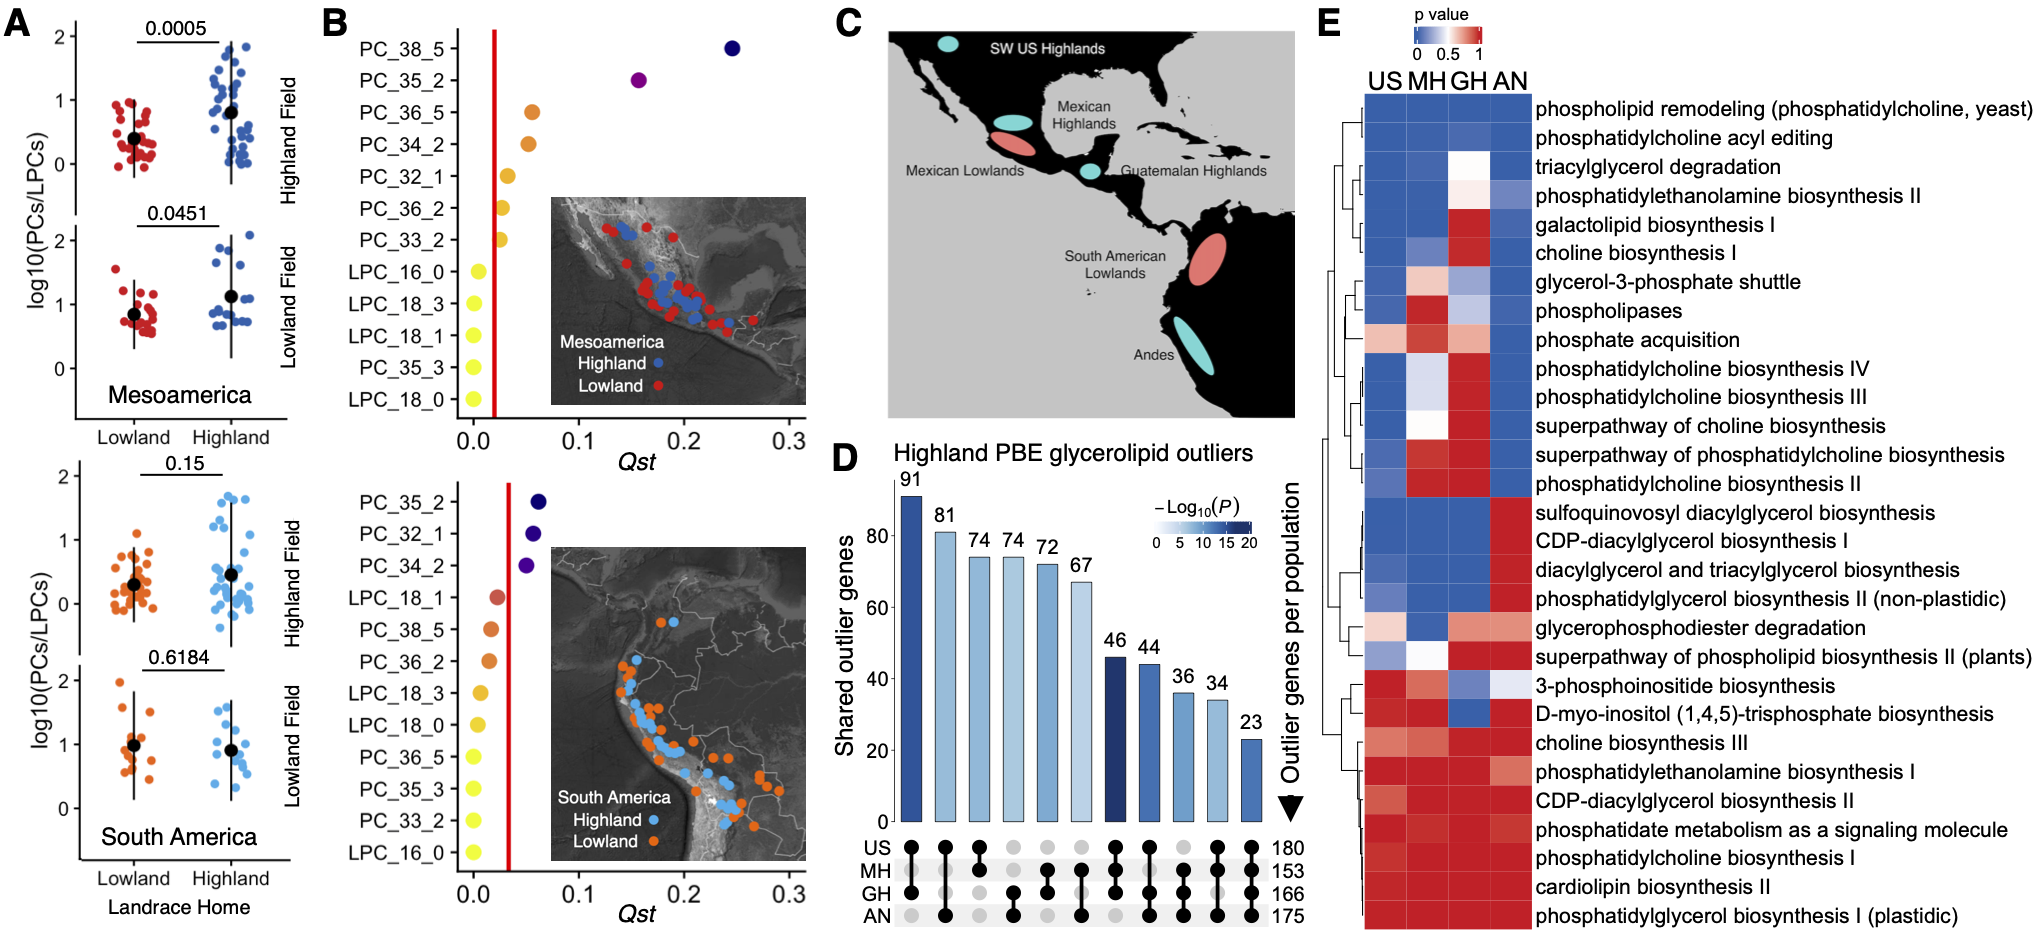
\includegraphics[width=0.4\paperwidth]{Figures/Fig_1.png}
\caption{\textbf{Phospholipid selection in highland maize.} 
\textbf{A)} Map showing the geographical origin of the 120 accessions from the HiLo diversity panel used in the common garden experiment to quantify glycerolipid levels.
\textbf{B)} PCs/LPCs ratio, in log scale, of highland and lowland landraces from MesoAmerica and South America, adjusted pairwise comparison t-test p-values shown.
\textit{$Q_{ST}$-$F_{ST}$} analysis of phospholipid compounds between highland and lowland landraces from Mesoamerica \textbf{C)} and South America \textbf{D)}.
} 
\label{Fig1}
\end{center}
\end{figure}

\begin{figure*}[ht]
\begin{center}
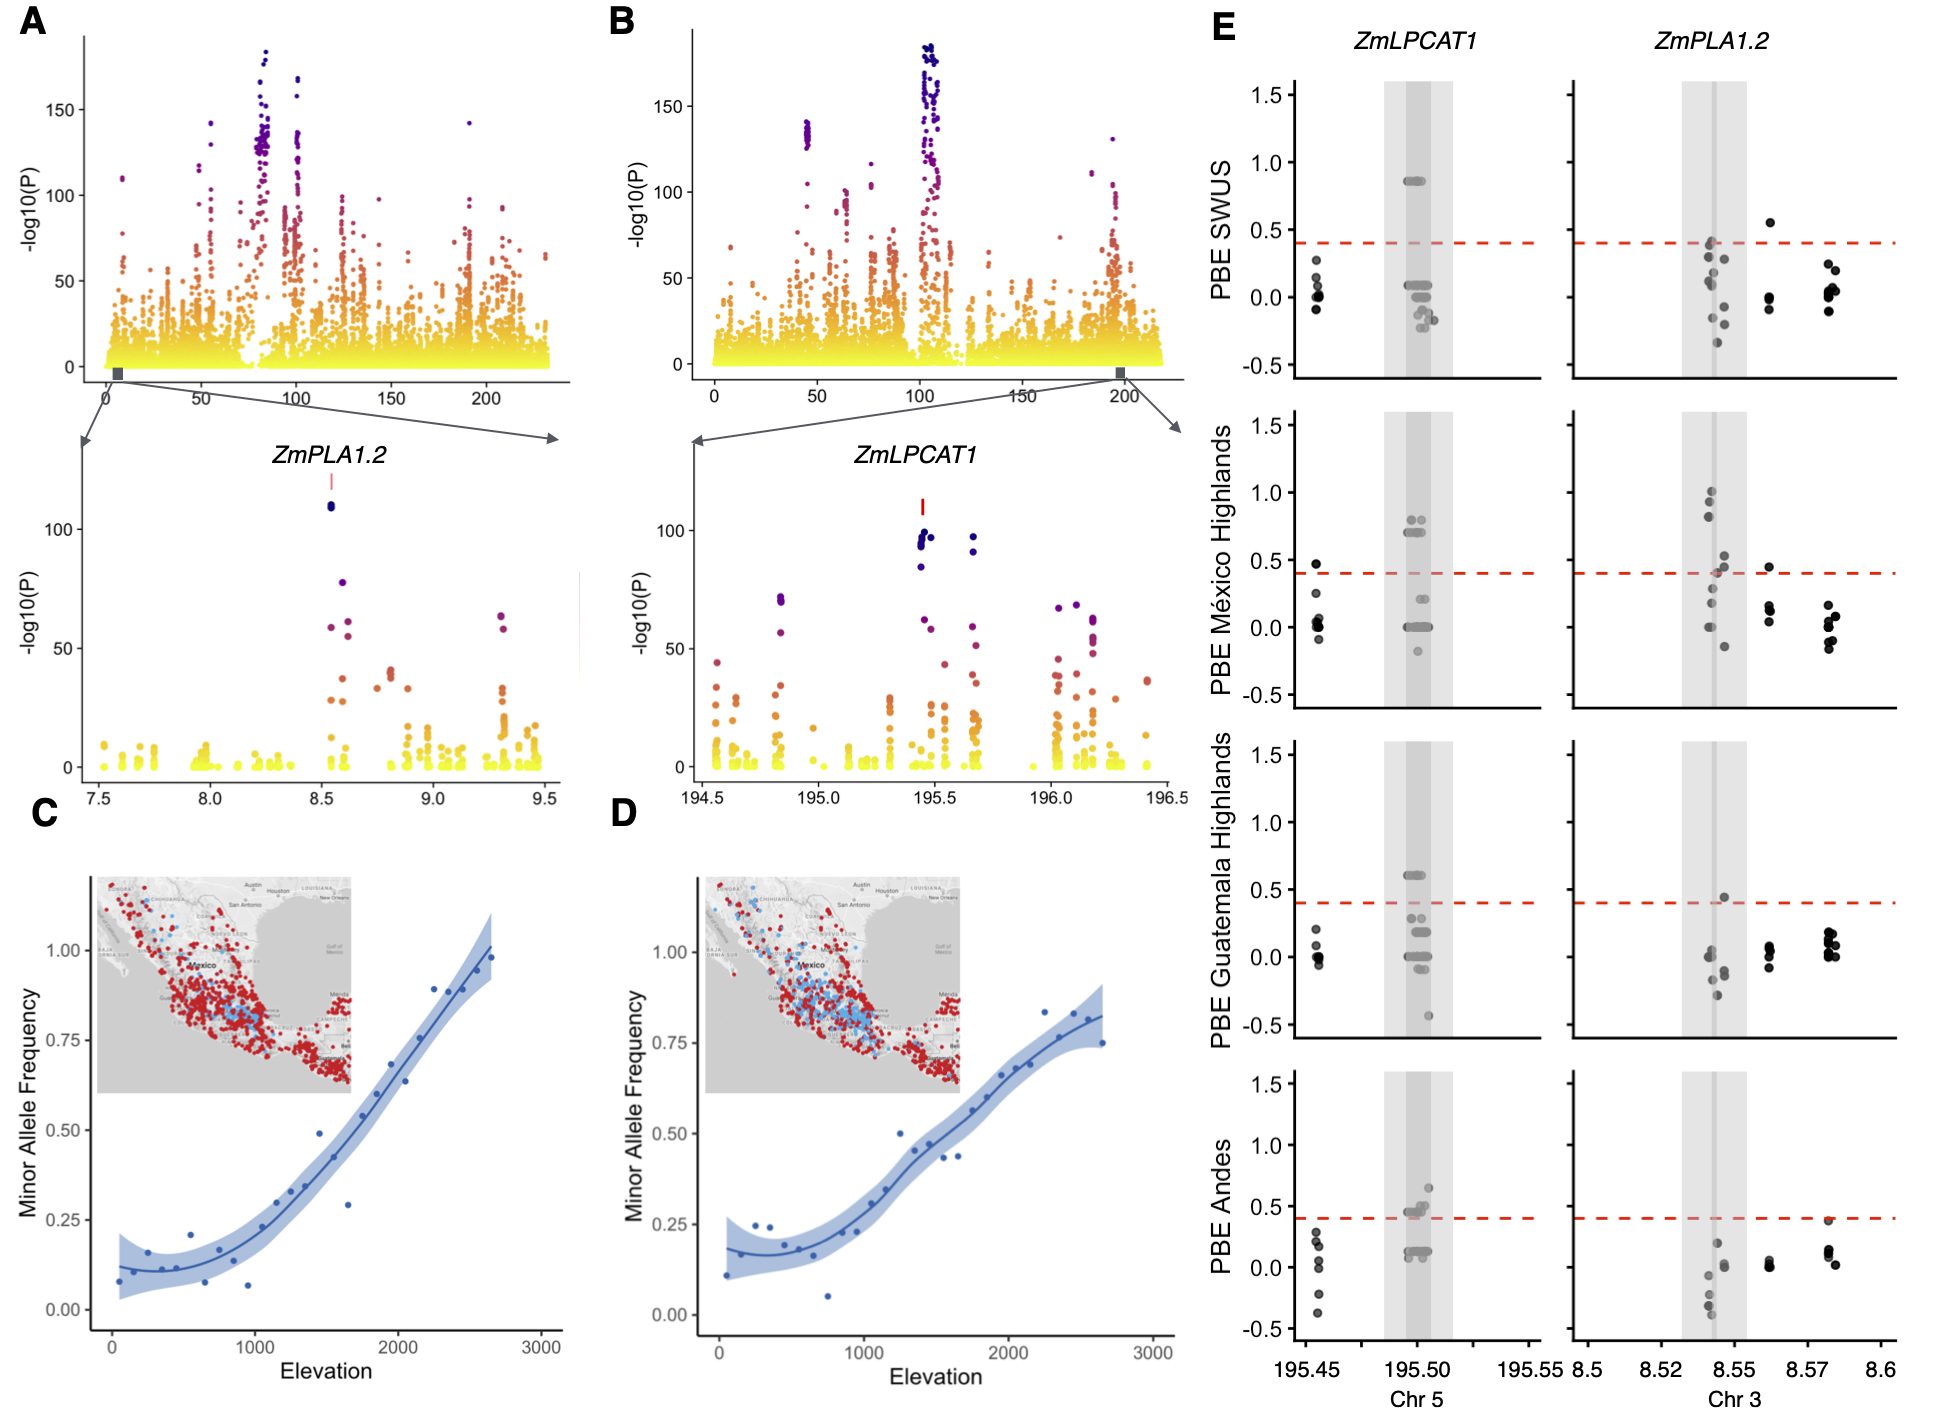
\includegraphics[width=0.6\paperwidth]{Figures/Fig_2.png}
\caption{\textbf{Highland selection in genes determining PC/LPC ratios.}
Manhattan plots of minus log10(P‐values) \textit{pcadapt} outliers. 
\textbf{A)} and \textbf{B)} \textit{pcadapt} PC1 outlier plots of chromosomes 3 and 5, respectively. 
Lower panels are zoomed areas of outlier SNPs that co-localize with the physical position of the coding sequences (marked with a red line) of \textit{HPC1} and \textit{ZmLPCAT1}. 
\textbf{C)} and \textbf{D)} show the geographic and elevation dependent minor allele frequencies of the highland (blue) and lowland (red) alleles of one of the outlier SNPs in the coding sequence of \textit{HPC1} and \textit{ZmLPCAT1}
\textbf{E)} PBE values of SNPs in \textit{ZmLPCAT1} and \textit{HPC1}}. 
\label{Fig2}
\end{center}
\end{figure*}

We grew a diversity panel composed of 120 highland and lowland landraces from Mesoamerica and South America (Fig. \ref{Fig1}A, Sup. File 1), hereafter HiLo diversity panel, in highland and lowland Mexican common gardens and quantified glycerolipid levels.    
We observed that Mesoamerican highland landraces showed  high PC/LPC ratios  particularly when grown in the highlands (Fig. \ref{Fig1}B).
The differences observed in phospholipid levels between highland and lowland maize could be the result of adaptive natural selection or random genetic drift during the process of maize colonization of highland environments.
To distinguish between these two competing scenarios, we compared each phenotype’s population variance with the genetic variance of neutral markers using a $Q_{ST}$-$F_{ST}$ comparison \cite{Leinonen2013-ic}.
We calculated $Q_{ST}$-$F_{ST}$ using DartSeq genotypic data from the same plants that were used to analyze glycerolipid levels, and we calculated the $Q_{ST}$-$F_{ST}$ values for each glycerolipid species for highland/lowland populations of each continent. 
Mean $Q_{ST}$ was greater than mean $F_{ST}$ in Mesoamerican and South American comparisons, though only the Mesoamerican comparison was significant (two-tailed t-test, $p$ = 0.00073; South American comparison $p$ = 0.12).
However, we observed several PC and LPC species with higher $Q_{ST}$ values than the neutral $F_{ST}$ in both sub continents (Fig. \ref{Fig1}C-D).
In particular, one of the species with the highest $Q_{ST}$ values in both continents is PC-36:5. 

\subsection{Selection on phospholipid pathway genes} 
We used Genotyping By Sequencing (GBS) data from 2700 Mexican maize landraces, generated by the SeeD project \cite{Romero_Navarro2017-cn, Gates2019-xu}, to run a \textit{pcadapt} analysis that detects how loci are contributing to patterns of differentiation between major principal components of genetic variation \cite{Luu2017-ws}.
The first principal component of \textit{pcadapt} polarized Mexican landraces based on elevation of the geographical origin of the landrace (Sup. Fig. \ref{SupFig1}A).
Using this first principal component we identified outlier SNPs across the genome that are significantly associated with landrace elevation and potentially involved in local adaptation (Sup. Fig. \ref{SupFig1}B).
We identified $\approx 600$ genes involved in glycerolipid metabolism (See Materials and Methods for details), and from those 85 contained SNPs that were \textit{pcadapt} PC1 outliers (top 5\% -log(P)) (Sup. File 2).
%Does this represent enrichment? Are there more glycerolipid genes than you would expect by chance?
\begin{figure*}[!ht]
\begin{center}
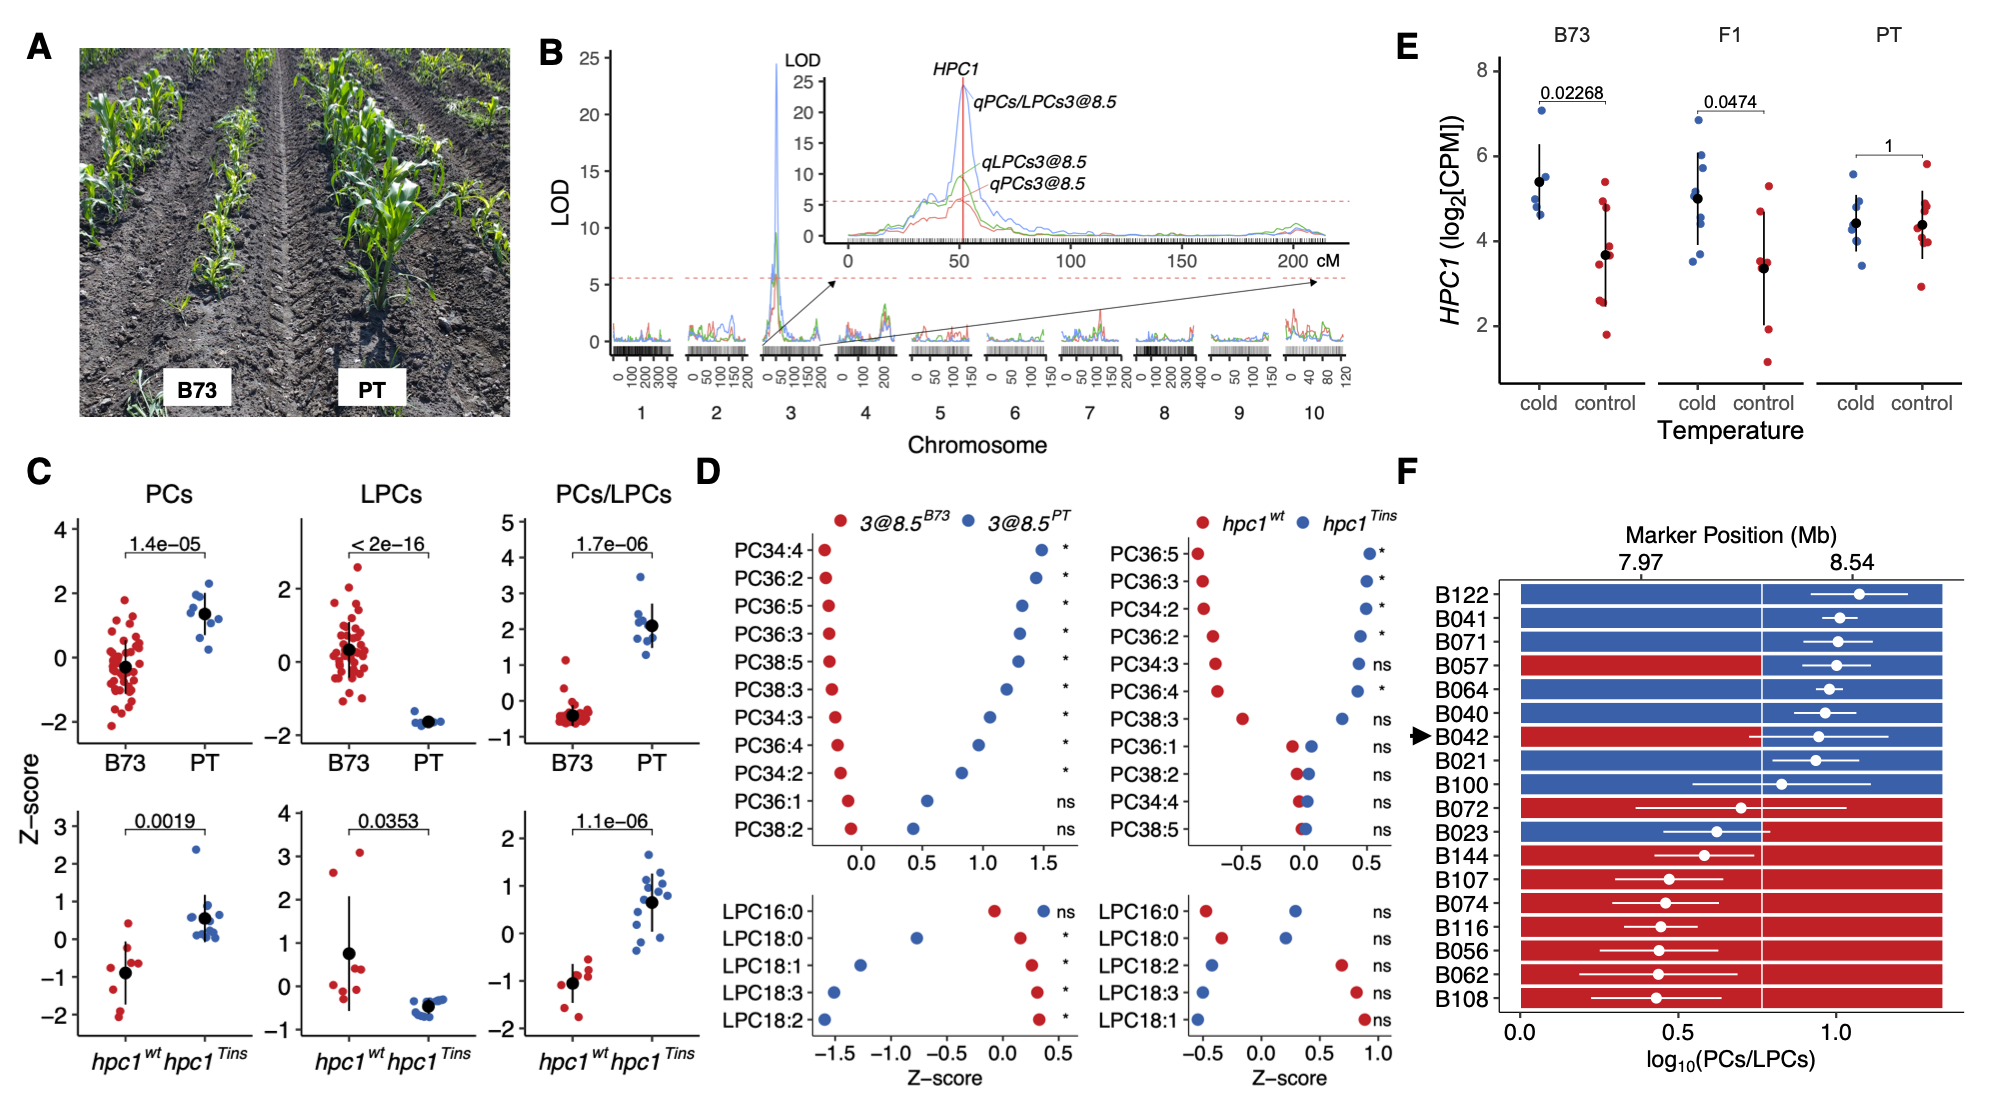
\includegraphics[width=0.8\paperwidth]{Figures/Fig_3.png}
\caption{\textbf{\textit{HPC1} is a major QTL explaining PC/LPC conversion.} 
\textbf{A)} PT and B73 plants growing in the highland Metepec field. 
\textbf{B)} QTL analysis using data collected from plants growing in the highland and lowland fields of PCs, LPCs and PCs/LPCs ratio identified overlapping major QTLs at 8.5 Mb in chromosome 3. 
QTL peak coincides with the physical location of \textit{HPC1}. 
\textbf{C)}PCs, LPCs and PC/LPCs z-scores effect sizes of RILs at chr 3 8.5 Mb that are either homozygous B73 or PT (top row) and CRISPR-CAS9 \textit{HPC1\textsuperscript{CR}} mutant and wild plants (bottom row).        
\textbf{D)} Individual PCs and LPCs species z-scores effect sizes of RILs at at chr 3 8.5 Mb (top row) and CRISPR-CAS9 \textit{HPC1\textsuperscript{CR}} mutant.
\textbf{E)} \textit{HPC1} expression analysis of B73, PT and their F1 grown in control and cold temperatures in growth chamber conditions.
\textbf{F)}PC/LPC ratios of several RILs including B042 that shows a recombination event 500 bp upstream of the ATG.}
\label{Fig3}
\end{center}
\end{figure*} 
We found that genes such as \textit{HPC1, High PhosphatidylCholine 1, Zm00001d039542} and \textit{ZmLPCAT1, Lyso-Phosphatidylcholine Acyl Transferase 1, Zm00001d017584} involved in phospholipid remodelling had SNPs within the coding sequence with significantly high -log(P) (Fig. \ref{Fig2}A-B) reflecting strong elevation-dependent allele frequency changes (Fig. \ref{Fig2}C-D). 
We then used the same set of 600 glycerolipid metabolism genes to identify selection signals using the Population Branch Excess (PBE) \cite{Pool2017-oa} statistic across four highland populations: Southwestern US (SWUS), Mexican Highlands (MH), Guatemalan Highlands (GH) and Andes \cite{Wang2020-mp}.
We found that, of the 153 glycerolipid-related genes that were PBE outliers in the Mexican Highlands, 38 were also \textit{pcadapt} PC1 outliers (Sup. File 2).
%Hufford: statistically  more overlap than expected?
There are two possible explanations for the extent of convergent selection in highland populations (see \cite{Wang2020-mp, yeaman2018}). 
Adaptation could be conferred by a small number of genes, thereby imposing a \textit{physiological} constraint on the sources of adaptation leading to convergence. 
On the other hand, adaptation could be encoded by a large number of genes, but deleterious \textit{pleiotropic} effects constrain the number of genes that can be targeted by selection, also leading to convergence.  
Using Yeaman's \textit{et al.} $C_{hyper}$ statistic \cite{yeaman2018} that quantifies these two modes of convergent adaptation, we found that the overlap among putatively adaptive genes in the four highland populations cannot be explained merely by physiological constraint ($C_{hyper} = 3.96$) and a certain degree of pleiotropic constraint is likely.
Overlap in adaptation candidates was higher for the SWUS MH and GH population pairs ($C_{hyper} = 4.79$), than between the Andean and SWUS MH and GH pairs ($C_{hyper} = 3.14$).
We identified a significant excess of genes that were targets of selection in more than two populations ($P< 3 \times 10^{-5}$, Sup. Fig. \ref{SupFig1}C).
The most over-represented intersection of selected glycerolipid genes was SWUS, MH, and GH ($p = 1  \times 10 ^{-15} $, Sup. Fig. \ref{SupFig1}C), perhaps indicating a set of genes specifically selected in this geographical region compared to the Andean material and/or closer kinship between those populations and therefore less statistical independence.
We found 22 genes from the glycerolipid pathways that were consistently PBE outliers in all four populations ($p =<1  \times  ^{-10}$, Sup. Fig. \ref{SupFig1}C). 
We then performed an independent analysis for each of the 30 pathways and compared the average pathway (10 Kb window around genes of that pathway) PBE value with a genome-wide genic random sampling distribution of PBE values. 
We found that 'phospholipid remodelling'  and 'PC acyl editing'  pathways had significantly high PBE values in all four populations indicating a possible role of phospholipid remodelling in maize highland adaptation (Sup. Fig. \ref{SupFig1}D and Sup. File 2). 
For example, \textit{ZmLPCAT1} is a selected gene  in the the 'phospholipid remodelling' and 'PC acyl editing' pathways that has shared outlier SNPs in the CDS region of all four populations (Fig. \ref{Fig2}E, Sup. File 2). 
\textit{HPC1} performs the reverse reaction of \textit{ZmLPCAT1} and is part of the 'PC acyl editing', 'triacylglycerol degradation' and 'phospholipases' pathways. 
\textit{HPC1} has particularly high PBE values in the Mexican highland population and contains SNPs that are unique for each population and others that are shared across populations (Fig. \ref{Fig2}E). 

\subsection{A major QTL explaining PC to LPC conversion overlaps with \textit{HPC1}} 
%Our PBE and glycerolipid analysis of multiple highland and lowland populations across the Americas showed a strong signature of selection in genes involved in the synthesis and degradation of phospholipids. 
%Glycerolipid analysis of the HiLo landrace diversity panel together with $Q_{ST}$-$F_{ST}$ results further supported that high PC/LPC ratios were selected for in highland maize from MesoAmerica and to a lesser extend in South America.
To break population structure and identify loci involved in phospholipid synthesis in highland maize, we developed a Recombinant Inbred Line (BIL) BC1S5 population from a cross between the temperate inbred line B73 and the Mexican highland landrace 'Palomero Toluqueño' (PT), using B73 as the recurrent parent (75\% B73, 25\% PT). 
\begin{figure*}[!ht]
\begin{center}
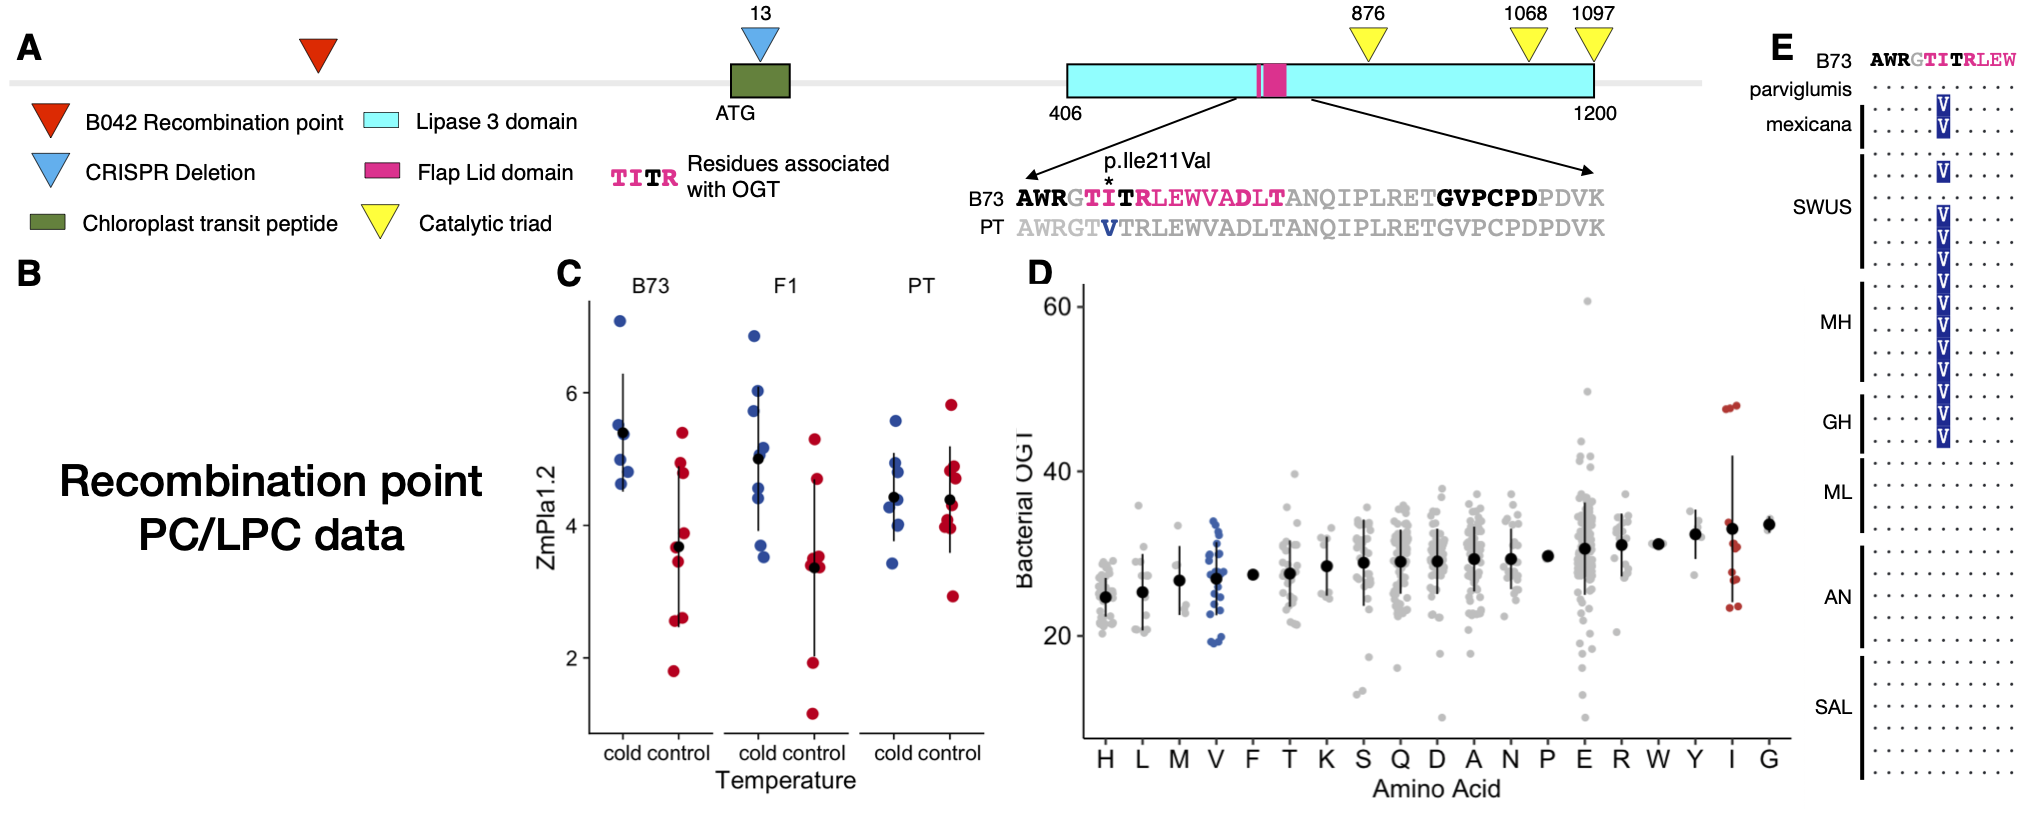
\includegraphics[width=0.8\paperwidth]{Figures/Fig_4.png}
\caption{\textbf{Fitness effects of \textit{HPC1-PT} and \textit{HPC1\textsuperscript{CR}}.} 
\textbf{A)} We used BLUPs and GBS data from ~ 2700 landraces from \cite{Gates2019-xu} evaluated in 23 common gardens at different elevations in México. 
We modeled each trait as a function of \textit{HPC1-PT} genotype, trial elevation, and tester line, with controls for main effects and responses to elevation of the genomic background. 
Gray lines and ribbons show estimates of the effect of the highland allele of \textit{HPC1-PT} as a function of common garden elevation ± 2SE, using the \textit{GridLMM} package \cite{Runcie2019-Gr}. 
Purple lines show estimates of the \textit{HPC1-PT} effect in a model that additionally included effects of Days-to-Anthesis. ASI, anthesis to silking interval
\textbf{B)} Flowering traits measured in the CRISPR-CAS9 \textit{HPC1\textsuperscript{CR}} mutant is long day conditions during the Summer of 2020 in Clayton, NC. 
CR represents CRISPR-CAS9 plants, WT represents wild-type plants, CR-WT represents the difference between the two. DTA is days to anthesis, DTS is days to silking.} 
\label{Fig4}
\end{center}
\end{figure*}
The parental PT accession is a popcorn (Palomero means popcorn in Spanish) from the Toluca Valley in México (\textit{Mexi5} CIMMYTMA 2233) (Fig. \ref{Fig3}A). 
The Hilo diversity panel and the B73 x PT BC1S5 mapping population were grown in the same highland and lowland common gardens and sampled for glycerolipid analysis.
Palomero Toluqueño, a locally adapted landrace, showed higher fitness than B73 in the highland field (Fig. \ref{Fig3}A), probably due to adaptation to low temperatures in the highland environments.  
In Mexican highlands values of around five growing degree units are typical while in lowland environments 15-20 GDUs are common. 
We found major QTLs for LPCs, PCs and PCs/LPCs at the same locus on chromosome 3 around 8.5 Mb (Fig. \ref{Fig3}B). 
The PCs/LPCs ratio QTL had the highest LOD (24.5) and percentage of phenotypic variance explained (87\%), while association with LPCs and PCs was not as strong (Sup. Table 2).
We searched for epistatic interactions in LPCs, PCs, and the PCs/LPCs ratio through a combination of R/qtl \code{scantwo} and \code{stepwise} functions \cite{Broman2003-ac}, but no additional QTLs were found.
These three summary QTLs, \textit{qLPCs3@8.5}, \textit{qPCs3@8.5} and \textit{qPCs/LPCs3@8.5}, were robust to environmental effects and we found them in either the highland or lowland data.
The additive effect of the PT allele at these QTLs leads to high levels of PCs, low levels of LPCs and consequently high PC/LPC ratios while the B73 allele has the opposite effect (Fig. \ref{Fig3}C, top panel).
Individual PC and LPC QTLs at this locus show the same additive PT allele effect behavior than the sum of each class of species \textit{qLPCs@8.5} and \textit{PCs3@8.5} (Fig. \ref{Fig3}C, top panel and Sup. Fig.\ref{SupFig2}). 
All individual LPC QTLs at the qLPCs3 locus correspond to LPCs that contain at least one double bond in the fatty acid (Sup. Fig \ref{Fig2}, Sup. file 3).
The summary \textit{qPCs3@8.5} was driven mainly by PC species with more than 2 fatty acid double bonds such as PC 36:5 (Fig. \ref{Fig3}D and Sup. Fig. \ref{SupFig2} bottom panel).

We then sought to identify candidate genes underlying the QTLs on Chr 3.
The QTL 7.9-10 Mb 1.5 LOD drop confidence interval contained 72 genes. 
We hypothesized that the metabolic phenotypes we observed could be due to a gene that is involved in the process of PC-LPC conversion.  
There are 75 genes in the maize genome with predicted phospholipase activity (Sup. Fig.\ref{SupFig3}A) and half of them have predicted phospholipase A1 activity (Sup. Fig.\ref{SupFig3}A).  
We identified \textit{HPC1} (Chr3:8,542,107..8,544,078), within the QTL peak, as the most likely candidate (Fig.\ref{Fig3}B). 
\textit{HPC1, High PhosphatidylCholine 1} has a predicted Phospholipase A1-Igamma1 activity and can be classified, based on its two closest \textit{Arabidopsis} orthologs (At1g06800 and At2g30550), as a PC hydrolyzing PLA1 Class I Phospholipase \cite{Ryu2004-iv}. 
PLA1 phospholipases hydrolyze phospholipids in the sn-1 position and produce a lyso-phospholipid and a free fatty acid as a result (Sup. Fig.\ref{SupFig3}B). 
Class I Phospholipases are targeted to the chloroplast and in fact we identified a Chloroplast Transit Peptide at the beginning of the CDS of the gene using ChloroP \cite{Emanuelsson1999-rs}.
We further confirmed chloroplast localization by transiently expressing  the \textit{HPC1} Chloroplast Transit Peptide fused with GFP in \textit{Nicotiana benthamiana} leaves (Sup. Fig. \ref{SupFig4}).
In B73, \textit{HPC1} is one of the most highly expressed phospholipases and its expression pattern is almost restricted to vegetative leaves (V4-V9) (Sup. Fig.\ref{SupFig5}A) \cite{Stelpflug2016-vr}, the same type of leaves that we sampled for glycerolipid analysis. 
In B73 leaf tissues, \textit{HPC1} is the most highly expressed gene of the QTL (7.9 - 10 Mb) (Sup. Fig. \ref{SupFig5}B \cite{Stelpflug2016-vr}).
%\textit{HPC1} is highly expressed in B73 and other temperate inbreds under low temperature conditions and is downregulated in heat conditions (Sup. Fig.\ref{SupFig5}C) \cite{Waters2017-nat}.
%Note: we decided to not talk about this in the results. We do mention it in the discussion.
%Our PBE and \textit{pcadapt} identified \textit{HPC1} as gene under strong selection in highland maize. 
%Our results in the landrace diversity panel also  indicated that the PCs/LPCs levels were particularly high Mexican highland landraces. 
%We further studied PC, LPC selection using the individual species and individual PC/LPC species ratio. 
%The ratio of PC to LPC is higher in RILs that are homozygous PT at the \textit{HPC1} locus. 
%The differences are most stark in ratios where the LPC lipid species is presumably a product of the reaction, as the reaction is not occurring in PT lines. 
%For example, \textit{HPC1} would remove a 16:0 fatty acid from PC34:1 and leave LPC18:1 behind. 
%Our PBE, \textit{pcadapt}, $Q_{ST}$-$F_{ST}$ and QTL data strongly suggest that the PC-LPC balance is under selection in highland Mexican maize and that \textit{HPC1}, and to a minor extent, \textit{ZmLPCAT1} are themselves under selection and are major drivers of the lipid changes observed in highland maize. 
%Furthermore, the QTL data suggest that the highland PT allele is a impairedfunction of \textit{HPC1}. 

\textit{HPC1} impaired function could be due to mis-regulation of \textit{HPC1} expression in highland landraces and/or to a mutation affecting the enzymatic activity of \textit{HPC1}. 
We analyzed \textit{HPC1} expression in B73, PT and the corresponding F1 in plants grown under high and low temperatures simulating highland and lowland conditions (Fig. \ref{Fig3}E). 
Under cold conditions \textit{HPC1-B73} was up-regulated but \textit{HPC1-PT} was not (Fig. \ref{Fig3}E). 
\textit{HPC1} in the F1 showed a pattern of expression consistent with a dominant B73 effect and this was also the case when we analyzed PC/LPCs ratios in the few B73 x PT BC1S5 RILs that are heterozygous at the \textit{qPC/LPC3@8.5} locus (Sup. Fig. \ref{SupFig3}C).
Impaired function could also be due to decreased enzymatic activity of the HPC1-PT variant and, in fact, PBE and \textit{pcadapt} outlier SNPs are located within the CDS of \textit{HPC1} and not within the regulatory region. 
We used Sanger sequencing to analyze three B73 x PT RILs (B021, B042, B122) that are homozygous PT at the \textit{HPC1} locus.
We identified a recombination point 500 bp upstream of the ATG of \textit{HPC1} (Fig. \ref{Fig3}F, Sup. Fig. \ref{SupFig6}) in RIL B042, resulting in a chimeric gene with the CDS from PT, and a promoter region from B73.
PC/LPC levels in the B042 RIL were similar to other RILs that are homozygous PT at the 8.54 Mb marker in the QTL peak (Fig. \ref{Fig3}F). 
This result supports the hypothesis that the metabolic effect we see is due to an impaired function of the HPC1-PT enzyme rather than changes in the \textit{HPC1-PT} regulatory region.
If \textit{HPC1} is the underlying causal gene of the QTL, the metabolic phenotypes observed would be consistent with a loss or impaired function of the \textit{HPC1-PT} allele that leads to higher levels of PCs and low levels of LPCs in PT. 
%This allele and the corresponding high PC/LPC ratio is conserved in other mesoamerican highland landraces (Fig.\ref{Fig1} and \ref{Fig2}). 
We generated a CRISPR-CAS9 \textit{HPC1} (\textit{HPC1\textsuperscript{CR}}) knockout mutant (Sup. File 4) in B104, a temperate inbred derived from B73, and measured PC and LPC species in WT and mutant plants grown under greenhouse control conditions. 
\textit{HPC1\textsuperscript{CR}} phenocopied the PT allele effect of the RILs (Fig. \ref{Fig3} C-D bottom panels), further confirming that the \textit{HPC1-PT} is an impaired function allele that underlies the QTL in chr3 @8.5 Mb. 

\subsection{Fitness effects of \textit{HPC1-PT}}
\textbf{\textit{HPC1} shows strong elevation-dependent antagonistic pleiotropy in Mexican landraces.} 
We re-analyzed phenotypic data from a previously-reported F1 Association Mapping panel \cite{Romero_Navarro2017-cn} \cite{Gates2019-xu}, fitting a model to estimate the effect of variation at \textit{HPC1-PT} on the relationship between fitness trait and elevation \cite{Runcie2019-Gr}. 
We found that variation at \textit{HPC1} significantly affected genotype-by-environment interaction for several fitness traits (Fig. \ref{Fig4}A). 
The effect of \textit{HPC1} on flowering showed antagonistic pleiotropy between highland and lowland environments (Fig. \ref{Fig4}A). 
The highland \textit{HPC1-PT} allele was associated with delayed flowering in lowland environments (an increase of around one day in days to anthesis (DTA)  and 1/4 of a day in the  Anthesis to Silking Interval (ASI)) but accelerated flowering at high elevation (a decrease of DTA and ASI of one and 1/4 of a day, respectively) (Fig. \ref{Fig4}A).
The effect of  variation at \textit{HPC1} on fresh ear weight and grain weight per hectare showed conditional neutrality: the highland allele had no effect in lowland environments but was associated with greater values in highland environments (Fig. \ref{Fig4}A).

\textbf{\textit{HPC1\textsuperscript{CR}} mutants phenocopied the effect of the highland allele on flowering time}.
We then grew the \textit{HPC1} CRISPR-CAS9 mutant in long-day conditions in North Carolina and measured flowering time. 
The \textit{HPC1\textsuperscript{CR}} mutant phenocopied the effect of the highland allele in Mexican lowland conditions and led to a delay in flowering time of around 1 day (Fig. \ref{Fig4}B) compared to wild-type plants. 

\textbf{Identification of the putative causal SNP in \textit{HPC1}.} We sequenced the \textit{HPC1} locus from several PT RILs and identified a number of non-synonymous SNPs within the CDS (407, 520, 553, 610, 631, 1028, 1315, 1342, and 1345 from the ATG) that could have an effect on HPC1 function.
We focused our attention on SNP 631 in the flap lid domain that leads to a conservative substitution of isoleucine for valine (V211I, Fig. \ref{Fig5}A).  
The flap lid domain is important for phospholipase activity and is located in a lipase 3 domain (PF01764) that is highly conserved across the tree of life. 
We recovered 982 observations of the lipase 3 PFAM domain from 719 prokaryote species using PfamScan \cite{Potter2018-tk, El-Gebali2019-pw}, and estimated optimal growth temperatures from their tRNA sequences \cite{Cimen2020-dm}.
We then tested if genetic variation in the lipase 3 domain was significantly associated with optimal growth temperature in bacteria. 
We found a number of significant associations, all of them located in the flap lid region (Fig. \ref{Fig5}A, bold letters).  
Interestingly, V at residue 211, the variant observed in the PT allele, was associated with lower bacterial optimal growth temperatures than the I seen in B73 (Fig. \ref{Fig5}B), suggesting the PT allele may be associated with adaptation to the low temperatures to which highland maize is exposed.

\begin{figure}[!ht]
\begin{center}
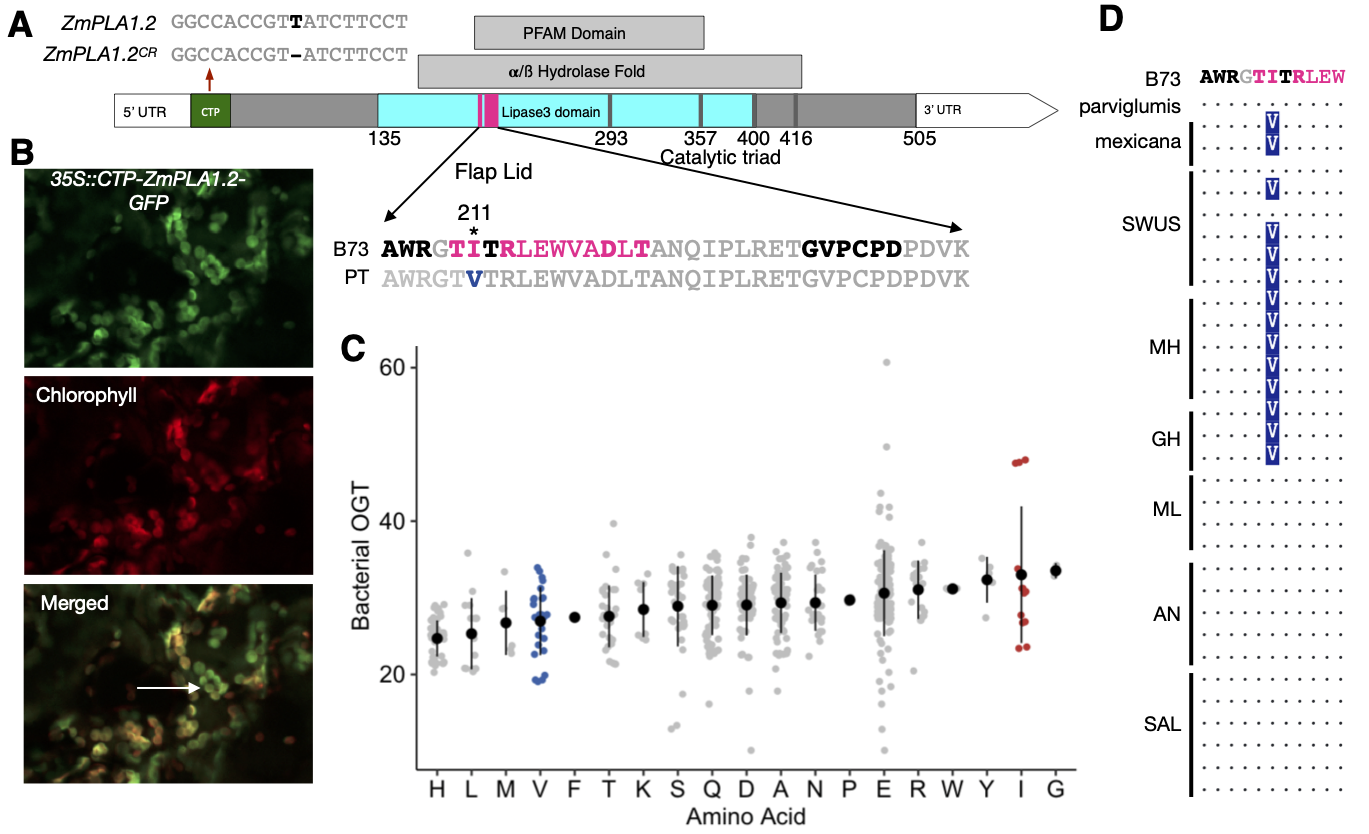
\includegraphics[width=0.4\paperwidth]{Figures/Fig_5.png}
\caption{\textbf{Analysis of \textit{HPC1} flap lid domain SNP effects.}  
\textbf{A)} \textit{HPC1} coding sequence showing different features. 
CTP represents the chloroplast transit peptide. 
Arrow in CTP indicates site of CRISPR-CAS9 deletion that leads to a premature stop codon.
Pink indicates residues of the flap lid domain.
Bolded residues showed significant associations with Prokaryote optimal growth temperature 
\textbf{B)} Prokaryote optimal growth temperature (OGT) of different residues at the 211 position}
\label{Fig5}
\end{center}
\end{figure}

\subsection{\textit{HPC1-PT} is an introgression from teosinte \textit{mexicana} and is conserved in Flint inbred lines} 
We then explored the segregation of the SNP leading to the V211I residue change among other highland maize varieties.
The PT allele was found at high frequencies in highland landraces from México and Guatemala and was segregating in Southwestern US landraces. 
The B73 allele was fixed in lowland Mexican, South American and Andean landraces (Fig. \ref{Fig6}A). 
These results are consistent with our previous PBE results (Fig. \ref{Fig2}E).
The PT allele was also present in teosinte, in 1/4 of the teosinte \textit{parviglumis} accessions and in both \textit{mexicana} accessions reported in Hapmap 3 \cite{Bukowski2017-ng} (Fig. \ref{Fig6}A). 
This led us to ask whether the PT allele was the result of post-domestication introgression from teosinte \textit{mexicana} during maize highland colonization or selected from \textit{parviglumis} standing variation.

\begin{figure*}[!ht]
\begin{center}
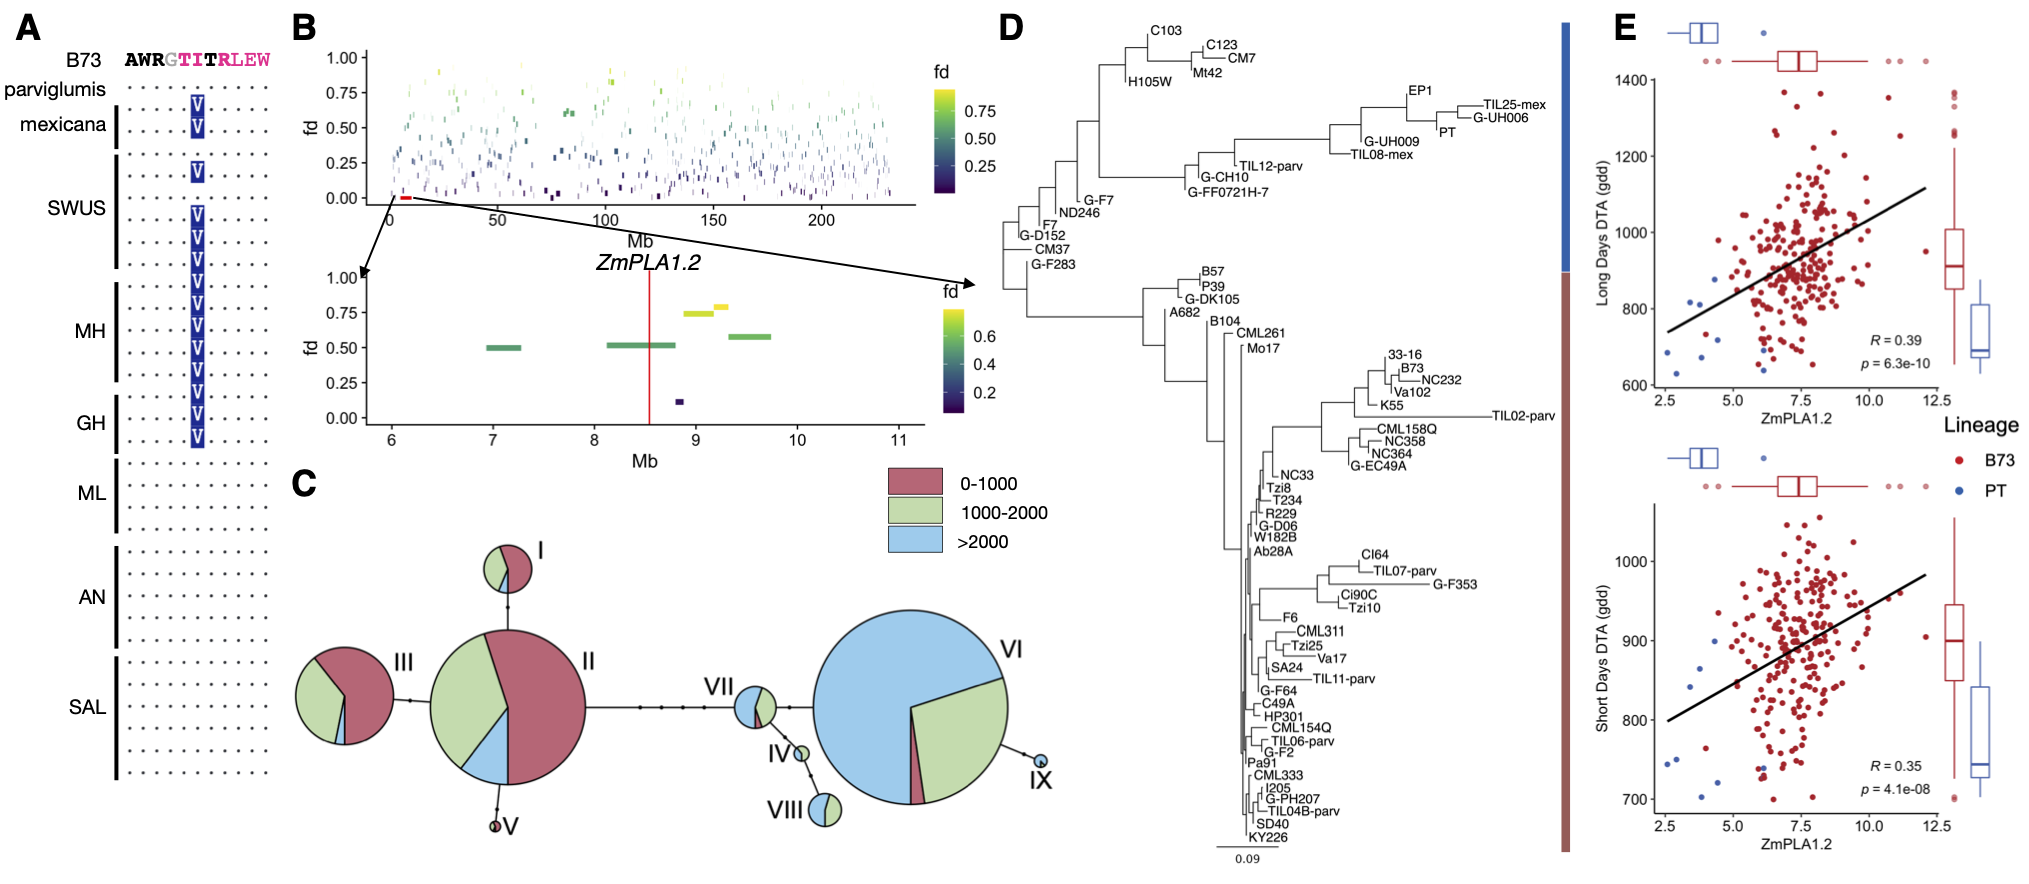
\includegraphics[width=0.8\paperwidth]{Figures/Fig_6.png}
\caption{\textbf{Introgression of teosinte \textit{mexicana} into maize \textit{HPC1}.}  
\textbf{A)} Alignments around the V211I mutation in the flap-lid domain in B73, \textit{mexicana} and \textit{parviglumis} and landraces of the Southwestern US, Mexico Highland and Lowlands, Guatemala Highlands, Andes and South America Lowlands.
\textbf{B)} \(f_d\) analysis of \textit{mexicana} introgression. Data were obtained from \cite{Gonzalez-Segovia2019-jy}. 
\textbf{C)} Haplotype network analysis of \textit{HPC1} CDS SNPs using 1060 Mexican homozyogous individuals from the SeeD dataset.
\textbf{D)} Cluster analysis of\textit{HPC1} CDS using a sample of Hapmap3 inbred lines and Palomero Toluqueño.
\textbf{E)} \textit{HPC1-PT} expression correlation with DTA in short and long days. 
Inbred lines from the PT lineage shown in panel C are colored in blue while inbred lines from the B73 lineage are colored in red,
data from \cite{Kremling2018-gn}}
\label{Fig6}
\end{center}
\end{figure*}

To test for \textit{mexicana} introgression, we used \(f_d\) data from \cite{Gonzalez-Segovia2019-jy} and found that the genomic region containing \textit{HPC1} showed signatures of introgression from \textit{mexicana} into highland maize (Fig. \ref{Fig6}B).
We then performed an haplotype network analysis using SNP data from the \textit{HPC1} CDS of 1160 Mexican accessions from the SeeD Dataset \cite{Romero_Navarro2017-cn} that were homozygous for all SNPS in the CDS and the teosinte inbred lines (TIL) from Hapmap 3 \cite{Bukowski2017-ng}.   
We identified nine haplotype groups that clustered mainly based on elevation (Fig. \ref{Fig6}C). 
The two major groups (II) and (VI) contained mainly lowland and highland landraces respectively. 
The two \textit{mexicana} teosinte inbred lines (TIL08 and 25) were located in group IV  (Fig. \ref{Fig6}C) together with highland landraces primarily collected in the Trans-Mexican Volcanic Belt (30/36 from the highlands of Jalisco, Michoacán, México, Puebla and Veracruz).
We then asked whether this \textit{mexicana} \textit{ZxHPC1} haplotype introgressed into Mesoamerican highland maize was also present in modern maize inbred lines. 
We performed a neighbor-joining cluster analysis using Hapmap 3 inbred lines including those from the 282 inbred panel, Teosinte Inbred Lines, German Lines and PT. 
We identified two main groups, one containing the \textit{HPC1-PT} haplotype and the other containing the \textit{HPC1-B73} haplotype.
Palomero Toluqueño and the teosinte \textit{mexicana}'s TIL-08 and TIL-25 clustered together with Northern European Flints like EP1, UH008, and UH009 (Fig. \ref{Fig6}D). 
Other Northern US flints like CM7 are also closely related to the \textit{mexicana} \textit{ZxHPC1} haplotype. 
These data suggest that after introgression into highland maize, the \textit{ZxHPC1} haplotype was conserved in Flint materials adapted to cold environments in the North of the US, Canada and Europe. 

Building on previous reports of a role for highly unsaturated PC species in determining flowering time \cite{Nakamura2014-qf, Riedelsheimer2013-bd} and considering the significant \textit{HPC1-PT} induced accumulation of those PC species, we asked if variation in \textit{HPC1} could be associated with differences in flowering time in modern maize. 
We used a large gene expression dataset obtained from the 282 maize diversity panel that was sampled at several developmental stages \cite{Kremling2018-gn}, and phenotypic datasets collected from the same panel grown in long- and short-day conditions.
We found that \textit{HPC1} and \textit{ZmLPCAT1} expression are inversely correlated in most tissues (Sup. Fig. \ref{SupFig7}), further supporting the idea that these two enzymes are co-regulated. 
There were significant associations between \textit{HPC1} expression in aerial tissues with several flowering time traits.
The magnitude of these associations was similar to those seen with other well characterized flowering genes (Sup. Fig. \ref{SupFig7}) such as \textit{ZmZCN8}  and \textit{ZmRAP2.7}.  
Furthermore, in both long- and short-day conditions, lines carrying the \textit{HPC1-PT} allele showed lower levels of expression and shorter flowering times than lines carrying the \textit{HPC1-B73} allele  (Fig. \ref{Fig6}E). 

 \section{Discussion}
\label{sec:discussion}
Understanding the genetic, molecular and  physiological basis of crop adaptation to different environments and the role that wild relatives have on these processes is relevant to identify favorable genetic variation that can be used to improve modern crops.
The repeated events of maize adaptation to highland environments constitute an excellent natural experiment to study crop local adaptation. 
Recent studies \cite{Wang2020-mp, Takuno2015-uj, Crow2020-gene} have helped improve our understanding of the genetics of maize highland adaptation. However, the molecular, physiological and genetic mechanisms of maize highland adaptation and the possible role of highland maize traits in modern, commercial varieties remains largely unknown.
Phospholipids are key structural components of plant membranes that also function as signaling molecules in adaptation to stresses prevalent in highland environments \cite{Ryu2004-iv, Nakamura2017-vb} such as low phosphorus availability \cite{Veneklaas2012-ls, Cruz-Ramirez2004-ib, Lambers2012-an} and low temperature \cite{Degenkolbe2012-wf, Welti2002-uk, Marla2017-ph}. 
Additionally, in Arabidopsis, accumulation of certain highly unsaturated phosphatidylcholine (PC) species can accelerate flowering time \cite{Nakamura2014-qf}, a major driver of maize adaptation to highland environments \cite{Romero_Navarro2017-cn, Gates2019-xu}.
 
Here we used genomic scans and linkage mapping to identify and clone \textit{HPC1, High PhosphatidylCholine 1} that encodes a phospholipase A1 enzyme that plays a major role in determining hosphatidylcholine levels in highland maize landraces.
We described that genetic variation on this locus shows strong antagonist pleiotropic G X E effects on several fitness traits.
We then show that the highland allele is the result of teosinte \textit{mexicana} introgression and that this introgression is conserved in modern maize inbreds adapted to high latitudes.
%that genes involved in the synthesis and degradation of PC species, such as \textit{HPC1} and \textit{ZmLPCAT1}, have been repeatedly selected in maize highland populations, leading to high PC/LPC ratios.   
%We then identified \textit{HPC1} as the gene underlying a major effect PC/LPC QTL in a B73 x Palomero Toluqueño RIL population. 
%The effect of the highland PT allele indicates it is impaired in function, possibly due to single point mutation in the flap-lid domain that reduces the efficiency of PC to LPC conversion. 
%The impact of genetic variation at \textit{HPC1} showed strong GxE effect with respect to elevation, delaying flowering in lowland environments but  accelerating flowering in highlands (Fig. \ref{Fig4}A).
%This effect was further confirmed in the CRISPR-CAS9 missense mutant, \textit{HPC1\textsuperscript{CR}}.
%We then found that the highland \textit{HPC1} haplotype is the result of teosinte \textit{mexicana} introgression that is still conserved in Northern USA, Canada and EU Flints. 
%Sequencing of the \textit{HPC1-PT} allele identified a SNP in the flap lid domain of the phospholipase that could probably affect substrate specificity and enzymatic activity.
%Indeed, a CRISPR KO mutant of \textit{HPC1} phenocopied the highland \textit{HPC1-PT} allele. 
%Evaluation of protein residue variation of the PFAM domain across hundreds of bacteria species further confirmed that the protein residue variation in the flap lid domain is associated with bacterial optimal growth temperature.
%We then found that the \textit{HPC1-PT} is conserved in Mexican and Guatemalan highland maize and to a lesser extent in Southwestern US maize and that this highland allele is the result of highland teosinte \textit{mexicana} into highland maize. 
%Moreover, the  \textit{ZxHPC1.2/HPC1-PT} haplotype is conserved in Northern US and European Flints and that lower expression of \textit{HPC1} is low in this Flint material and is correlated with faster flowering times.
%Finally, using phenotypic and genotypic data of thousands of Mexican accessions grown in several common garden trials across Mexico we show that genetic variation of \textit{HPC1} shows a strong G x E interaction where the highland allele leads to a delay of flowering time in lowland environments and an acceleration of flowering time in highland environments. 
%Other fitness related phenotypes show a similar G X E interaction where the highland \textit{HPC1} leads to more fit plants in highland environments and less fit plants in lowland environments. 
%This effect was confirmed using a CRISPR mutant of \textit{HPC1}.
%Our data indicate that \textit{HPC1} is a major component of the phpospholipid makepup of maize that can influence several fitness phenotypes important in maize adaptation to low temperatures through physiological and molecular mechanisms that will need to be further investigated.
%Given the important role of this environmental factors and plant traits in highland environments, we hypothesized that phospholipid metabolism has been important in the repeated events of maize highland adaptation. 
%We studied selection of pathways involved in glycerolipid metabolism (that includes phospholipids but also other non-phosphorus containing polar lipids such as galactolipids) at the genetic pathway level using a Population Branch Excess approach \cite{Pool2017-oa, Wang2020-mp}. 

We found that genes of pathways involved in the synthesis and degradation of phospholipids were repeatedly selected in several highland maize populations of North America, Central America and South America (Fig.\ref{Fig1} and \ref{Fig2} ). 
%These results are similar to other pathways that are known to be important for highland adaptation such as flowering time \cite{Wang2020-mp}. 
%Furthermore, our analysis of the modes of convergence \cite{yeaman2018} indicate that to a certain extent convergence across the different populations is explained by pleiotropic constraint similarly to what we have found in the same populations \cite{Wang2020-mp}.
\textit{ZmLPCAT1} and \textit{HPC1} were two of the genes that showed strongest, repeated signals of selection measured by PBE and \textit{pcadapt} in highland populations (Fig. \ref{Fig2}). 
A previous study found that \textit{ZmLPCAT1} showed high \textit{Fst} values when comparing highland and lowland landraces \cite{Takuno2015-uj}.
The predicted function of ZmLPCAT1 is to synthesize PC species via the acylation of LPC species while the predicted function of HPC1 is to hydrolyze PCs into LPCs and free fatty acids by cleaving at the sn1-position.
Selection in these two genes is probably driving the high PC/LPC ratio that we found in highland Mexican landraces (Fig.\ref{Fig1}).
%SNPs in the coding regions of \textit{ZmLPCAT1} and \textit{HPC1} genes were also strong outliers in the first \textit{pcadapt} principal components (that captures elevation dependent genetic variation) analysis of thousands of accessions across México (Fig. \ref{Fig2} and Sup. \ref{SupFig2}. 
%Phospholipid selection in highland maize was also reflected in phospholipid levels and \textit{Qst-Fst} values of phospholipid levels measured from plants of a landrace panel containing highland and lowland landraces grown in a common garden experiments in highland elevations of Mexico and (Fig.\ref{Fig1}D-E, Sup. \ref{SupFig1}C-D). 
Natural variation in maize \textit{HPC1} is associated with lipid content \cite{Riedelsheimer2012-bx} and flowering time \cite{Chen2012-gg, Hung2012-ms}. 
In B73, \textit{HPC1} is one of the most highly expressed phospholipases and its expression pattern is almost entirely restricted to vegetative leaves (V4-V9) (Sup. Fig.\ref{SupFig3}C) \cite{Stelpflug2016-vr}, the same type of leaves that we sampled for glycerolipid analysis. 
In B73 leaf tissues, \textit{HPC1} is the most highly expressed gene in  the QTL interval (7.9 - 10 Mb) (Sup. Fig. \ref{SupFig5}B \cite{Stelpflug2016-vr}).
Additionally, \textit{HPC1} is highly expressed in B73 and other temperate inbred lines under low temperature conditions and is down-regulated in heat conditions (Sup. Fig.\ref{SupFig3}D) \cite{Waters2017-nat}.
In our experiments, B73 and the B73 x PT F1 were up-regulated in cold conditions, while the expression of PT showed similar levels than B73 in control conditions, it was not up-regulated in cold conditions (Fig. \ref{Fig3}E).
In Arabidopsis, \textit{LPCAT1} is involved in the determination of phosphorus leaf content levels under low Zn conditions \cite{Kisko2018-zm}.
In maize a GWAS hit 45 KB upstream of \textit{ZmLPCAT1} for flowering time under low phosphorus conditions further supports the possible role of natural variation of \textit{ZmLPCAT1} in plant adaptation to low phosphorus availability. 
We are currently exploring if \textit{ZmLPCAT1} elevation dependent genetic variation could be involved in adaptation could be involved in highland maize adaptation to low phosphorus availability.

Our QTL analysis of PC/LPC ratios in a B73 x PT mapping population and in the \textit{HPC1\textsuperscript{CR}} mutant support the hypothesis that the highland \textit{HPC1-PT} allele results in an impaired function enzyme that alters highland Mexican maize PC metabolism leading to high PC/LPC ratios (Fig.s \ref{Fig3}). 
Using the PC/LPC ratio we obtained much more significant LOD QTL signals than we used PC or LPC levels alone, probably because the ratio can much more precisely capture genetically induced changes in enzymatic activity acting that determine metabolite ratios \cite{Petersen2012-ii}.
Adaptive loss of function mutations can be an effective way to gain new metabolic functions in new environmental conditions \cite{Hottes2013-np}. 
Our data support an enzymatic impaired function due to a single conservative amino acid substitution located in the flap lid domain of HPC1 that can impact substrate  accessibility and/or substrate binding (Fig.\ref{Fig5}A). 
%This single SNP leads to amino acid change the 211 position from isoleucine in B73 to valine in PT (Fig.\ref{Fig4}a.
%This is a conservative substitution, but can potentially have a big impact in substrate accessibility and/or substrate binding. 
%Residue 211 is also associated with lower optimal growth temperature in bacteria than the Zm-PLA-B73 residue (Fig.\ref{Fig4}D).
%Moreover, we found that genetic variation of residues in or around the flap lid domain, not just 211, Fig.(\ref{Fig4}A, bold letters) is associated with optimal growth temperature in bacteria and archaea. 
Indeed, the flap lid domain has been the target of biotechnological modification of these types of enzymes \cite{Khan2017-ua}.

Why were the metabolic changes induced by HPC1 selected in highland maize?
PC metabolism is intimately connected to multiple stress response and developmental pathways; alterations in PC amounts and PC/LPC ratios impact overall plant fitness.
%After domestication in the the tropical lowlands of Southwestern México, maize expanded throughout the Americas and adapted to environmental conditions that are very distinct from the original site of domestication.
%Today maize is  cultivated on all five continents and used for a myriad of culinary and industrial purposes. 
%Understanding the evolutionary, metabolic and physiological mechanisms that enable made to adapt to new environments is relevant both from an agronomical and basic evolutionary genetics point of view.
%In this paper we focused our attention on the role of phospholipid metabolism in the multiple events of maize adaptation to highland environments in the Americas and their
%It can be difficult to compare lipid changes across studies, as the time of day the sample is taken, intensity of stress applied, and initial growth environment of the plants can impact the outcome of the lipid analysis \cite{Kenchanmane_Raju2018-nz}. 
%Despite these caveats, lipid changes in response to low temperature have been well studied. 
%We observe similar trends between cold-acclimation-imposed lipid changes published in the literature and adaptation-imposed lipid changes in highlands maize. 
The \textit{qPC/LPC3@8.5} QTL is driven by individual QTLs of PC and LPC species with high levels of unsaturated fatty acids (Sup. Fig. \ref{SupFig2}).
Some of these species, like PC 36:5 and LPC 18:1  (Fig.\ref{Fig3}D, Sup. File 3), show similar patterns during Arabidopsis cold acclimation \cite{Welti2002-uk} and sorghum low temperature response \cite{Marla2017-ph}.
PC 36:5 also showed high $Q_{ST}$ values when comparing highland and lowland landraces from both Mesoamerica and South America (Fig. \ref{Fig1}C-D, Sup. File 5).
%Increases in PC 36:5 and 36:6 combined with decreases in LPC 18:1 of highland maize resemble observed PC and LPC changes that occur during Arabidopsis cold acclimation \cite{Welti2002-uk} and sorghum chilling response \cite{Marla2017-ph}.
%Highland maize shows an increase in PC and decrease of LPC. This trend is matched in Arabidopsis responding to cold acclimation where PC 36:5 and 36:6 increases, while LPC 18:1 decreases \cite{Welti2002-uk}. PC 36:5 and 36:6 increasing during cold stress also occurs in sorghum \cite{Marla2017-ph}. 
%When exploring the lipid changes, they found that maize and sorghum, two relatively cold-sensitive species, displayed increases in desaturation in PC, while tripsacum, the relatively cold-tolerant species, displayed decreases in PC desaturation \cite{Yan2019-tx}. 
%The desaturation increase in total PC is matched in a separate sorghum chilling study, as well \cite{Marla2017-ph}. 
In maize, \textit{HPC1} expression shows circadian regulation\cite{Khan2010-iv} and peaks at the end of the day. 
%During light hours, \textit{HPC1} transcript increases, and during dark hours, it decreases. 
%Lipids have long been known to fluctuate in response to time of day \cite{Browse1981-vt, Ekman2007-xe}. 
%with specific fatty acids like 16:1, 16:2, and 18:0 highest at the end of the light cycle and 16:3 highest at the end of the dark cycle. 
In Arabidopsis, highly unsaturated PC (34:3, 34:4, 36:5, 36:6) species increase during the dark\cite{Maatta2012-ip}, coinciding with low expression levels of \textit{PLA1.2}\cite{Khan2010-iv}.
Furthermore, Yuki Nakamura and colleagues elegantly showed that PC 36:5 and 36:6 species accumulate during the night and can bind to Arabidopsis flowering time locus T (FT) accelerating flowering time \cite{Nakamura2014-qf} by cellular mechanisms still not well understood. 
The Arabidopsis FT ortholog in maize, \textit{ZCN8} \cite{Lazakis2011-nq}, underlies a major flowering time and photoperiod sensitivity QTL \cite{Hung2012-ms}.
Additive mutations in the regulatory region of \textit{ZCN8}, including a teosinte \textit{mexicana} introgression, lead to higher expression of \textit{ZCN8} contributing to maize adaptation to long days in temperate conditions \cite{Guo2019-pn}.
Our results show that HPC1 drives the accumulation of PC species (such as PC 36:5) that accumulate in Arabidopsis at the end of the day and that can bind to FT and accelerate flowering time. 
We hypothesize that accumulation of these PC species in highland maize could drive early flowering in a similar way that occurs in Arabidposis. 

The effect of genetic variation of \textit{HPC1} on flowering time in Mexican landraces indicated a strong GxE interaction where the highland allele lead to a reduction of flowering time and ASI in highland environments (Fig. \ref{Fig4}A) similar to the effect observed to the well known teosinte \textit{mexicana} introgression of inversion \textit{inv4m} \cite{Crow2020-gene}.
Other flowering time loci analyzed do not show this clear GxE effect \cite{Gates2019-xu}.
Interestingly, the effect of the highland allele shows typical conditional neutrality in yield-related traits, with increased fitness of the \textit{HPC1-PT} allele in highlands (Fig. \ref{Fig4}A).

The flap-lid mutation in HPC1-PT residue 211 is conserved in highland Mexican and Guatemalan landraces and in teosinte \textit{mexicana} (Fig. \ref{Fig6}A) but is still segregating in teosinte \textit{parviglumis}. 
We showed that indeed, \textit{HPC1-PT} is an introgression from teosinte \textit{mexicana} (Fig. \ref{Fig6}B) and that this introgression has been conserved in modern inbred lines particularly northern US, Canada and EU Flints (Fig. \ref{Fig6}D). 
\textit{HPC1} in inbred lines carrying the \textit{ZxHPC1} \textit{mexicana} haplotype show low levels of expression and earlier flowering times (Fig. \ref{Fig6}E) \cite{Kremling2018-gn}. 
Other grasses such as \textit{Tripsacum dactyloides} adapted to temperate latitudes also show accelerated rates of evolution in genes involved in PC metabolism \cite{Yan2019-tx}.
Moreover, genetic variation in the regulatory region of \textit{HPC1} was significantly associated with photoperiod sensitivity in the maize Nested Association Mapping population \cite{Hung2012-ms}. 

In summary, here we used a combination of genomic scans, linkage mapping, lipidomics and reverse genetics to identify and clone an adaptive teosinte \textit{mexicana} introgressed gene \textit{HPC1} in highland maize landraces that leads to a major reorganization of phosphatydilcholine metabolism. 
We showed that fitness advantage of the \textit{HPC1} highland allele is at least due to its effect in accelerating flowering.

%Conversely, LPC increases at the end of the light period when \textit{HPC1} is the most highly expressed.
%Maatta et al 2012 reports that PC in Arabidopsis cycles in this manner \cite{Maatta2012-ip}. PC 34:3, 34:4, 36:5, and 36:6 are all higher at 11 hours into the dark period. 
%Connecting this to the HPC1 expression from Khan 2010, it would be plausible that the lack of HPC1would be one component allowing for an increase in PC during the dark. 
%Continuing this trend, LPC 18:1 is also significantly higher at the end of the light period, when HPC1 expression is also the highest. 
%PC 36:5 and 36:6 not only accumulate during the night, but also bind to Flowering Locus T(FT)\cite{Nakamura2014-qf}.
%Nakamura et al, 2014 showed that PC is intimately tied to flowering as the Arabidopsis protein Flowering locus T (FT) binds to PC in vitro \cite{Nakamura2014-qf}. 
%Transgenically increasing PC levels in the shoot apical meristem of Arabidopsis caused a faster flowering time, while lowering them caused flowering delays. 
%The ortholog of FT in maize is ZCN8  ZCN8 underlies a major flowering time QTL and regulatory changes in ZCN8 through various SNPs have allowed maize to adapt its flowering time \cite{Guo2019-pn}.
%However, it is not yet known if ZCN8 also has the ability to bind to PC.

%\section{Significance statement} 
%After domestication in the tropical lowlands of México, maize expanded throughout the Americas and adapted to very diverse environments. 
%Because of its rich evolutionary history, maize is an ideal species to study convergent evolution. 
%Here, we use multiple highland adapted populations to study how phosphatidylcholine metabolism helped maize adapt to new environments. 
%We show that an introgression from teosinte \textit{mexicana} \textit{HPC1} into maize lead to an increase in phosphatidylcholine levels that improved maize fitness probably through an effect on flowering time.  
%\textit{HPC1} is a good example of what could be many genes to be characterized in the \textit{mexicana} introgression that may help maize adapt to stressful growing conditions. 

\section{Materials and Methods}
\label{sec:materials:methods}
\textbf{Populations used in the analysis.} 
Highland and lowland populations used for Population Branch Excess analysis consisted of three to six accessions from each of the highland and lowland populations and have been previously described in \cite{Wang2020-mp, Wang2017-bc}. 
The 120 Landraces from the HiLo diversity panel were selected and ordered from the \href{http://mgb.cimmyt.org/gringlobal/search.aspx}{CIMMYT germplasm bank} to maximize a good latitudinal gradient sampling across Mesoamerica and South America. 
For each highland landrace (>2000 masl) a lowland landrace (<1000 masl) was selected at the same latitude (<0.5\degree) to form 60 highland/lowland pairs, 30 from each continent. 
The list of the accessions used is provided in Sup. file 1.   
B73 x Palomero Toluqueño Recombinant Inbred Lines (RILs) were developed by crossing B73 with a single Palomero Toluqueño plant (Mexi5 accession, CIMMYTMA 2233) that was then backcrossed with B73 once and selfed five times (BC1S5).  
We used  individual landrace accession genotype and fitness data from the CIMMYT Seeds of Discovery project (SeeD) \cite{Gates2019-xu} to calculate \textit{pcadapt} \cite{Luu2017-ws} values and GxE effects of \textit{HPC1-PT}.

\textbf{Field Experimental Conditions and sampling.} 
Two replicates of the HiLo diversity panel accessions and three replicates of the B73 x PT RILs were planted in a highland and lowland common gardens. 
The highland common garden was located in Metepec, Edo de México, (19\degree13'28.7"N 99\degree32'51.6"W) in the Trans-Mexican volcanic belt. 
The field is at 2610 meters above sea level (masl), and the range of average monthly temperatures along the year vary from 5 \degree C to 21.5 \degree C.  
The lowland common garden was located in Valle de Banderas, Nayarit, (20\degree47'01.2"N 105\degree14'47.0"W) in the Pacific Coast. 
The field is at 50 meters above sea level (masl), and the range of average monthly temperatures along the year vary from 20 \degree C to 29 \degree C.
Between growth stages V4 and V6, we used a leaf puncher to collect 50 mg of fresh tissue (10 discs) from the tip of the second leaf above the last leaf with a fully developed collar. 
Tissue discs were immediately flash frozen in liquid nitrogen. 
We collected all samples from a field in a single day between 10:00 am and 12:00 pm, approximately 3 h after sunrise. Samples were transported in dry ice to the lab and stored at -80\degree C until extraction. 

\textbf{Glycerolipid analysis} 
We crushed frozen samples in a tissue grinder Retsch (Haan, Germany) for 40 seconds at a frequency of 30 1/s. 
We performed lipid extraction following Matyash and collaborators \cite{Matyash2008-ue}. 
First, we added 225 $\mu$L of cold methanol (MeOH) to each sample. 
For the blanks, we prepared MeOH containing a Quality Control (QC) mix (Sup. File 6).
We vortexed each sample for 10 seconds, keeping the rest of the material on ice. 
Then, we added 750 $\mu$L of cold methyl tert-butyl ether (MTBE). 
For the blanks, we used MTBE containing 22:1 cholesterol ester as internal standard (Sup. File 6). 
We vortexed each sample for 10 seconds, followed by 6 minutes of shaking at 4\degree C in the orbital mixer. 
We next added 188 $\mu$L of LC/MS grade water at room temperature (RT), and vortexed samples for 20 seconds.
We centrifuged the samples for 2 min at 14000 rcf and recovered 700 $\mu$L of supernatant from the upper organic phase. 
We then split the supernatant into two aliquots of 350 $\mu$L, one aliquot was used for the generation of the lipid profile and the other aliquot was used to prepare pools that were used along the lipid profiling. 
Finally, we dried the samples using a speed vacuum concentration system.
We resuspended dried samples in 110 $\mu$L of MeOH-Toluene 90:10 (with the internal standard CUDA, 50 ng/mL). 
We vortexed samples at low speed for 20 s and then sonicated at RT for 5 min. 
We then transferred aliquots of 50 $\mu$L per sample into an insert within an amber glass vial.
The UHPLC-QTOF MS/MS utilized were Agilent 1290 and Agilent 6530, respectively. 
We used a Waters Acquity charged surface hybrid (CSH) C18 2.1x100 mm 1.7 $\mu$m column which we initially purged for 5 min. 
We coupled the UHPLC column with a VanGuard pre-column (Waters Acquity CSH C18 1.7$\mu$m). 
We injected six “no sample injections” at the beginning of each run to condition the column, followed by ten samples, one pool (made out of the mix of the second aliquot of all the samples contained per UHPLC plate) and one blank.
We injected 1.67 $\mu$L per sample into UHPLC-QTOF MS/MS ESI (+); the running time per sample was 15 min. 
Mobile phase “A” consisted of 60:40 acetonitrile:water, 10 mM of ammonium formate and 0.1\% formic acid. 
Mobile phase “B” consisted of 90:10 isopropanol:acetonitrile, 10 mM ammonium formate and 0.1\% of formic acid. 
The flow rate was 0.6 mL/min and the column compartment was maintained at 65° C. Initial conditions were 15\% B; the gradient uniformly increased until reaching 100\%. 
At 12.10 min the mobile phase composition returned to initial conditions.
We used the mass spectrometer (Q-TOF MS/MS) in positive electrospray ionization mode (ESI).
The source parameters were: ESI gas temperature 325 \degree C, nebulizer pressure 35 psig, gas flow 11L/min, capillary voltage 3500 V, nozzle voltage 1000V, and MS TOF fragmentor and skimmer 120 and 65 V, respectively.
We used a mass range between 60 and 1700 m/z, under acquisition parameters. 
As for reference mass parameters, we used a detection window of 100 ppm and a minimum height of 1000 counts. 
We performed a retention time (rt) correction of the acquired data using Agilent MassHunter Qualitative Analysis B.06.00 version and Microsoft Excel. 
To extract ion chromatograms (EICs) of the internal standards within the run we used Agilent MassHunter Qualitative Analysis.
We identified the time of the highest intensity point of each EIC, which we used as the current retention time of the experiment. 
We used the method retention time for internal standards and the current rt and we fitted a polynomial regression to calculate new retention times using retention times from 501 lipids of a MS1 m/z-rt library (See Sup. File 7). 
In MSDIAL \cite{Tsugawa2015-kh}, identification of lipids is based on two approaches: the MSP file and MS/MS identification setting included in MSDIAL and the use of a post identification file containing accurate m/z and rt for a list of lipids. 
In this study we used both identification approaches. 
Under positive ion mode, the MSP file and MS/MS identification setting has a total of 51 lipid classes  selectable for identification. 
The post identification file that we used was the retention time-corrected MS1-MS2 mz-rt lipid library that we explained before. 
We used MSDIAL \cite{Tsugawa2015-kh} version 3.40. 
To use MSDIAL, we converted the raw data from .d to .abf format with Reifycs Abf converter (https://www.reifycs.com/AbfConverter/). 
Then, we filtered the MSDIAL alignment results based on whether compounds intensity was ten times above blank intensity. Next, filtered data were normalized using Systematic Error Removal using Random Forest (SERRF) \cite{Fan2019}. This normalization is based on the quality-control pool samples. 
We filtered out, now the normalized features, considering a coefficient of variation (CV) equal or less than 30\% among the pools. 
To curate the data for duplicate features, isotopes and ion-adducts, we utilized MS-FLO \cite{DeFelice2017-ms}.
We also normalized the curated data using the sum of all known metabolite signal (mTIC). 
After data processing and normalization, we used lipid intensities for further analysis.

\textbf{CRISPR-CAS9 Glycerolipid analysis}
Dry samples were resuspended in 110 $\mu$L of 100\% MeOH (with the internal standard CUDA, 50 ng/mL), vortexed at low speed for 20 s and then sonicated at RT for 5 min. 
We transferred the samples into amber glass vials with inserts prior to analysis. 
Lipid profiling was performed using a Thermo Scientific Orbitrap Exploris 480 mass spectrometer coupled to a Thermo Vanquish Horizon UHPLC. Chromatographic separation was achieved using the same guard and analytical column type, mobile phase composition and gradient conditions described for UHPLC-QTOF analyses. 
Avanti Splash Lipidomix Mass Spec Standard (Avanti Polar Lipids, Alabaster, Alabama) was used to check system suitability and a Lipid QC Standard Mixture (Sup. File 6) and pooled QC samples were used to monitor instrument performance. 
Methanol solvent blanks were injected at the beginning of the sequence and throughout the batch between approximately 10 injections and pooled QC samples were injected between every 6–8 sample injections. For ion source parameters the spray voltage was set at 3500 V, sheath gas 60 (arb), aux gas 15 (arb), sweep gas 2 (arb) and ion transfer tube and vaporizer temp at 350 \degree C. 
Full scan and data-dependent MS/MS (ddMS\textsuperscript{2}) scans were collected in positive ESI mode following 2 $\mu$L sample injections. 
Full scan spectra were obtained from \textit{m/z} 220-1700 using an Orbitrap resolution setting of 120000, RF lens set at 25\%, normalized AGC target at 25\% and maximum injection time set to auto. 
ddMS\textsuperscript{2} scans were performed using a cycle time of 0.6 s, intensity threshold of 5.0e4, and a 3 s dynamic exclusion using a 10 ppm mass tolerance. 
Additional parameters for ddMS\textsuperscript{2} experiments were as follows: Isolation window equal to 1 Da, stepped collision energy at 20 and 30\%, Orbitrap resolution set to 15000, scan range set to auto, normalized AGC target of 100\% and a maximum ion injection time of 55 ms. 
Data files were uploaded to LipidSearch 4.2.2 (Thermo Scientific, Tokyo, Japan) for identification of PC and LPC species. 
Skyline-daily \cite{Adams2020-em} was then used to obtain normalized peak areas for the identified PCs and LPCs using the internal standards PC(12:0/13:0) and LPC(17:0), respectively.

\textbf{$\mathbf{Q_{ST}-F_{ST}}$ analysis of glycerolipid data.}
Quantitative trait differentiation ($Q_{ST}$) was contrasted to the distribution of $F_{ST}$ for neutral genetic markers \cite{whitlock2008evolutionary}.
Highland/Lowland contrasts were considered separately for Mesoamerica and South America.
A linear mixed effects model (R package lmer, function lmer) was used to partition phenotypic variance between population pairs (Mesoamerica/South America, all highland/all lowland, Mesoamerican highland/Mesoamerican lowland, South American highland/South American lowland).
\begin{center}
${ TRAIT \sim 1 + (1|POPULATION) + }$\\
${(1|GARDEN/BLOCK) + (1|BATCH)}$
\end{center}
Within-population and between-population variances were calculated with the R function VarCorr (R package \texttt{lme4}, \citealp{bates2014lme4}), and were used to calculate $Q_{ST}$ following the equation below:
\begin{center}
$Q_{ST}$ = \(\sigma^{2}_{GB}/(\sigma^{2}_{GB}+2\sigma^{2}_{GW})\)
\end{center}
\noindent in which $\sigma^{2}_{GB}$ and $\sigma^{2}_{GB}$ are the between- and within-population genetic variance components, respectively \cite{Leinonen2013-ic}.
Pairwise $F_{ST}$ was calculated with the R function fst.each.snp.hudson (R package \textit{dartR}, \citealp{gruber2018dartr}).

\textbf{\textit{pcadapt} analysis of biological adaptation in Mexican landraces.}
In order to conduct genome scans for signatures of adaptation we used the \textit{pcadapt} \cite{Luu2017-ws} package.
\textit{pcadapt} identifies adaptive loci by measuring how strongly loci are contributing to patterns of differentiation between major axes of genetic variation.
Under simple models \textit{pcadapt} captures major patterns of $F_{ST}$  but is conducted in a way that does not require population delimitation \cite{duforet2014genome}.
As the genome scan comparison requires a focal SNP to be compared to the first K principal components of the genotype data, it can be biased by large regions of low recombination that drive the major axes of variation in the principal components.
Thus, when SNPs from these low recombination regions are compared against principal components driven by linked loci spurious signals may arise.
To prevent this bias from occurring, we used custom scripts to calculate the principal component step separately based upon all the chromosomes except for the chromosome of the focal SNPs being tested.
The genotype data we used for this analysis was GBS data from roughly 2,000 landraces of Mexican origin collected by CIMMYT (www.cimmyt.org) as part of the SeeDs of discovery initiative (https://www.cimmyt.org/projects/seeds-of-discovery-seed/).
From this, we calculated the strength of association between each SNP and the first five principal components (excluding the chromosome of the focal SNP) using the communality statistic as implemented in \textit{pcadapt} version 3.0.4.

\textbf{Glycerolipid pathways selection.}
We compiled a list of genes pertinent to glycerolipid metabolism starting with a search of all genes belonging to the \textit{Zea mays} 'Glycerophospholipid metabolism' and 'Glycerolipid metabolism' KEGG pathways \cite{kanehisa2019} (map identifiers: zma00564 and zma00561). 
With the NCBI Entrez gene identifiers in KEGG we retrieved the AGPv4 transcript identifiers used in Corncyc 8.0 \cite{portwood2019, walsh2016} from an id cross reference \href{https://www.maizegdb.org/search/gene/download_gene_xrefs.php?relative=v4}{file} found in MaizeGDB   \cite{portwood2019}.
This resulted in a list of 300 genes comprising 51 Corncyc pathways. 
Then we discarded Corncyc pathways  tangentially connected to the KEGG glycerolipid metabolism list (sharing just one enzyme with the initial KEGG list) or that we judged to belong to different biological processes (e.g 'long chain fatty acid synthesis','anthocyanin biosynthesis'). 
Finally, we added manually the 'phosphatidylcholine biosynthesis V' pathway that was missing. 
The list of 30 selected Corncyc pathways included genes outside the initial KEGG search results and raised the number of genes to 557. 
In addition to this, 37 genes were found to have an enzymatic activity related to phospholipid metabolism but not placed into any particular pathway, i.e orphan enzymes, consisting mostly of alcohol dehydrogenases. 
Sixteen additional genes found in KEGG were not annotated at all in Corncyc probably due to differences between AGPv4 and RefSeq pseudogene annotation of the maize genome. 
The list of all possible candidates coming either from KEGG or Corncyc that were orphan enzymes or were unannotated in Corncyc amounted to 594 genes (Sup. File 2). 
This process is documented in the \verb|0_get_glycerolipid_genes.R| script of the \verb|pgplipid| R package accompanying this paper \cite{fausto_rodriguez_zapata_2020_4323410}.

\textbf{Population Branch Excess Analysis.}
Population Branch Excess quantifies changes in allele frequencies in focal populations relative to two independent “outgroup” populations.
We used \textit{Zea mays spp. parviglumis} as one of the outgroup populations for all four highland groups.  
The other outgroup was  Mexican Lowlands  in the case of Southwestern US , Mexican Highlands and Guatemalan Highlands; and South American Lowlands in the case of the Andes population. 
We used calculated PBE SNP values for the 4 populations (described in detail in \cite{Wang2020-mp}) and we tested for selection outliers SNPs in the 594 phosphoglycerolipid candidates and the 30 Corncyc pathways (556 genes).
We first defined PBE outlier SNPs as the top 5\% of the PBE score distribution; this fraction corresponds to approximately 50000 out of ~1 million genotyped SNPs in each population. 
Following \cite{Wang2020-mp}, we defined a gene as a PBE outlier if it contained an outlier SNP within the coding sequence or 10 Kbp upstream/downstream. 
Then we tested for over-representation of genes selected in particular subsets of populations using Fisher's exact test with the 32283 protein genes from the maize genome as background. 
For each pathway, we first selected all SNPs within CDS regions and 10Kb upstream and downstream of genes in the pathway and we calculated the mean pathway PBE score. 
We then constructed a null distribution by drawing 10000 samples without replacement of $n$ SNPs from those found within or around 10Kb upstream and downstream of all protein coding genes and we obtained the mean PBE for this null distribution. 
%Jeff: this is a weird permutation. you have n snps in x genes. you then randomly draw n SNPs from the 32283 genes, but very likely end up representing snps from >>x genes. You need to 1) count each gene once not  each window  (see comment above) and 2) draw from genes as the permutation, not SNPs then 3) ask whether the genes you draw contain an outlier SNP. this still isn't perfect -- ideally you draw x genes and subsample n snps but  probably not worth  doing that
%For each pathway, the heat map shows p-values corresponding to the probability of sampling from the null distribution a set of $n$ SNPs with the observed glycerolipid pathway mean PBE score or higher.
With the set of PBE outliers for glycerolipid metabolism in the 4 populations we tested for evidence of physiological or pleiotropic constraint using the $C_\chi^2$ statistic \cite{yeaman2018}. 

\textbf{QTL analysis of phospholipid levels.}
We analyzed glycerophospholipid QTLs in a mapping population of 57 RILs (BC1S5) from the cross B73 x PT.
These RILs were grown in a highland site in Metepec, Edo de México at 2600 masl during the Summer of 2016 and in Puerto Vallarta, Jalisco at 50 masl during the Winter of 2016/17.  
We analyzed the samples using UHPLC-QTOF, as above, and 67 leaf lipid species were identified.
For QTL analysis we calculated the mean across all fields of individual lipid mass signal. 
We also used as phenotypes the sum total of the following lipid classes: diacylglycerol, triacylglycerol, PC and  LPC.  
Furthermore,  we also included the log base 10 transformed ratios of LPCs/PCs and the ratios of their individual species. 
We did a simple single marker analysis  with ``scanone`` using Haley-Knott  regression, and assessed the QTL significance with 1000 permutations.

\textbf{CRISPR-CAS9 editing of \textit{HPC1} and analysis of the effect of \textit{HPC1\textsuperscript{CR}} mutant on flowering time.}
CRISPR/Cas9 was used to create a \textit{HPC1} gene knockout through \textit{Agrobacterium} mediated transformation of background line B104 \cite{Wu2020-nq, Char2017-uk}. 
RNA guides were designed as described in \cite{Brazelton2015-co} for the B73 reference genome v4. 
B104 and B73 sequence for \textit{HPC1} were identical. 
The gRNA cassette was cloned into pGW-Cas9 using Gateway cloning. 
Two plants from the T0 transgenic event were identified through genomic PCR amplification and Sanger sequencing and were self-pollinated. 
In the next generation several plants were further selfed.
Plants were genotyped using forward primer CAGTTCTCATCCCATGCACG and reverse primer CCTGATGAGAGCTGAGGTCC.
Homozygous \textit{HPC1\textsuperscript{CR}} T2 plants were  planted for lipid analysis in greenhouses at  North Carolina State University during Spring 2020 and then self-pollinated. 
Cas9 positivity was tested for using 0.05\% Glufosinate ammonium contained in Liberty herbicide. 
Wild type plants from the same segregating families were used for analysis.

\textbf{Effect of \textit{HPC1\textsuperscript{CR}} mutant on flowering time.}
T3 CAS9-free plants were grown in isolation during summer 2020 in Clayton, NC. 
Female (Days to Silking) and male (Days to Anthesis) flowering time were calculated from the day of planting until the first silks and anther pollen shed could be observed in each individual plant. 
Plants homozygous \textit{HPC1\textsuperscript{CR}} and WT derived from the same T1 families were planted for this experiment. 
Effect size analysis was performed using the dabestR package \cite{Ho2019-yl}.

\textbf{Expression analysis of \textit{HPC1} in B73, PT and B73xPT F1s in conditions simulating highland environments.}
Gene expression data were generated from leaf tissue from B73, PT and the B73xPT F1. 
Plants were grown following the same protocol as in \cite{Crow2020-gene}.
Briefly, kernels were planted in growth chambers set to imitate spring temperature conditions in the Mexican Lowlands (22$^{\circ}$C night, 32$^{\circ}$C day, 12 hr light) and highlands (11$^{\circ}$C night, 22$^{\circ}$C day, 12 hr light). 
Leaf tissue was sampled from the V3 leaf the day after the leaf collar became visible, between 2 and 4 hours after lights came on. Tissue was immediately placed in a centrifuge tube, frozen using liquid nitrogen, and stored at -70$^{\circ}$C.

RNAseq libraries were constructed, sequenced, and analyzed following \cite{Crow2020-gene}. 
Briefly, randomly primed, strand specific, mRNA-seq libraries were constructed using the BRaD-seq \cite{townsley2015brad} protocol.
Multiplexed libraries were sequenced on 1 lane of an Illumina HiSeq X. 
Low quality reads and adapter sequences were removed using Trimmomatic v.0.36 \cite{bolger2014trimmomatic}, and the remaining paired reads were aligned and quantified using \texttt{kallisto} v.0.42.3 \cite{bray2016near}. 
Gene counts were normalized using the weighted trimmed mean of M-values (TMM) with the \textit{calcNormFactors} function in \textit{edgeR} \cite{robinson2010edger} and converted to log2CPM.

\textbf{Sanger sequencing of \textit{HPC1} in RILs homozygous at the \textit{qPC/LPC3@8.5} locus.}
We identified 3 RILs homozygous for the PT allele at the \textit{HPC1} locus and we developed 6 sets of primers to Sanger sequence across the CDS and the gene promoter. 
The location of primers in the gene are shown in Sup. file 8. 

\textbf{Association of \textit{HPC1} with agronomic traits}.
We re-analyzed phenotypic data from the F1 Association Mapping (FOAM) panel of Romero-Navarro \textit{et al} \cite{Romero_Navarro2017-cn} and Gates \textit{et al} \cite{Gates2019-xu} to more fully characterize association signatures of \textit{HPC1}. 
Full descriptions of this experiment and data access are described in those references. 
We downloaded BLUPs for each trait and line from Germinate 3, and subset the data to only those lines with GBS genotype data from México. 
We fit a similar model to the GWAS model used by \cite{Gates2019-xu} to estimate the effect of the \textit{HPC1-PT} allele on the traits' intercept and slope on trial elevation, accounting for effects of tester ID in each field and genetic background and family effects on the trait intercept and slope using four independent random effects. 
We implemented this model in the \textit{R} package \textit{GridLMM} \cite{Runcie2019-Gr}. 
We extracted effect sizes and covariances conditional on the REML variance component estimates and used these to calculate standard errors for the total \textit{HPC1-PT} effect as a function of elevation. 
To test whether the phenotypic effects of \textit{HPC1-PT} on yield components could be explained as indirect effects via flowering time, we additionally re-fit each model using Days-To-Anthesis as a covariate with an independent effect in each trial.
%\textbf{Phosphorus analysis and phosphorus soil availability data.}
%We analyzed phosphorus content in B73 and 5 Mexican  and 5 Peruvian highland landraces (Sup. file 10) grown in control field conditions in the 2018 Puerto Vallarta, México, Winter nursery. 
%Samples were analyzed using ICP-MS according to \cite{Baxter2014-ch}. 
%Frequency of Andosol soils at different elevations was calculated using the soilP package \cite{Rodriguez-Zapata2018-vz}. %Jeff: feels weird here. 
%Phosphorus content in flag leaves of the the same \textit{HPC1\textsuperscript{CR}} and WT mutants used for the flowering time experiment were analyzed using ICP-OES at the North Carolina Department of Agriculture.

\textbf{Identification of features and domains of \textit{HPC1}.}
The domains of \textit{HPC1} were analyzed from UniProt identifier \hyperlink{https://www.uniprot.org/uniprot/A0A1D6MIA3}{A0A1D6MIA3}. 
The \hyperlink{https://www.ebi.ac.uk/interpro/entry/pfam/PF01764/}{Lipase3-PFAM - PF01764}, and \hyperlink{https://www.ebi.ac.uk/interpro/entry/InterPro/IPR029058/}{alpha/beta Hydrolase fold} were identified using InterPro, and \hyperlink{https://www.ncbi.nlm.nih.gov/Structure/cdd/cddsrv.cgi?uid=cd00519}{Lipase3-CDD}, shown in cyan, including flap lid, shown in magenta, and S293, D357, and H400 catalytic triad were identified from CDD. 
H416 was identified as a substitute for H400 in the catalytic triad by protein modelling.

\textbf{Bacterial optimal growth temperature association with HPC1 flap-lid domain allelic variation}.
We compared the maize \textit{HPC1} protein sequence to prokaryotes with the same sequence to determine whether the identified residue change in maize and accompanying association with low temperature survival was consistent with observations in other organisms. 
We identified the Pfam domain PF01764 in the B73 protein sequence using the HMMER3 web server, we also identified 982 observations of the PF01764 Pfam domain in 719 prokaryote species using PfamScan \cite{Potter2018-tk, El-Gebali2019-pw}. 
We predicted the optimal growth temperature of these species using tRNA sequences as in \cite{Cimen2020-dm}. 
We aligned the maize and prokaryote PF01764 domain sequences with hmmalign from the hmmer3 package \cite{Eddy2011-pd}, and the aligned Pfam sequences were recoded to reflect nine amino acid physicochemical properties \cite{Li2016-ut}. 
We filtered the sequences to remove gaps in the domain alignment and observations with only partial domain sequences, then we clustered based on sequence similarity, resulting in two clusters of observations within the domain. 
For each cluster, positions in the filtered alignment were associated with prokaryote optimal growth temperatures using a linear regression with all 9 amino acid physicochemical properties. 
Seventeen sites in and around the flap-lid region of the protein passed a 10\% FDR significance threshold, including the single residue change Ile211Val previously identified in \textit{HPC1-PT}. 
Welch’s two-sided t-test was used to compare the optimal growth temperatures of prokaryote species with the \textit{HPC1-B73} allele to the optimal growth temperatures of prokaryote species with the \textit{HPC1-B73} allele at this site.

\textbf{Subcellular localization of \textit{HPC1}.}
We fused the HPC1-B73 Chloroplast Transit Peptide (52 aminocacids) with GFP. %Jeff: no idea what this is saying
Three constructs encoding subcellular localization signals were used as control; Cytoplasm (C-GFP), nucleus (N-GFP), and Chloroplast (P-GFP). 
All of them were under control of the 35S promoter. 
These constructs were transiently expressed in \textit{Nicotiana benthamiana} leaf cells.

\textbf{Teosinte \textit{mexicana} introgression in highland maize.}
To evaluate if the \textit{HPC1-PT} allele was the result of standing variation from teosinte \textit{parviglumis} or introgression from \textit{mexicana} we used Patterson's \textit{D} statistic and genome-wide $f_{d}$ to calculate ABBA-BABA patterns. 
The data were obtained from \cite{Gonzalez-Segovia2019-jy}. 
The material used in \cite{Gonzalez-Segovia2019-jy} included whole genome sequence data from three highland outbred individuals: two Palomero Toluqueño and one Mushito de Michoacán; three lowland landraces: Nal Tel (RIMMA0703) and Zapalote Chico (RIMMA0733) obtained from \cite{Wang2017-bc} and  BKN022 from \cite{Bukowski2017-ng}; two \textit{mexicana} inbred lines: TIL08 and TIL25; three \textit{parviglumis} inbred lines: TIL01, TIL05, TIL10 and \textit{Tripsacum} TDD39103 \cite{Bukowski2017-ng} as an outlier. 

\textbf{Haplotype network analysis of \textit{HPC1} in Mexican maize landraces and teosintes.}
We extracted SNP genotypes for \textit{HPC1} from the TIL teosinte accessions in the HapMap 3 imputed data \cite{Bukowski2017-ng} and the 3700 Mexican landraces in the SeeD dataset. 
With the set of 1060 accessions that were homozygous at all sites in this genomic region we calculated a haplotype network depicting the minimal spanning tree for haplotypes covering 90\% of the input accessions with the R package \code{pegas} \cite{paradis2010}, and haplotype frequencies for three elevation classes in the landraces (0-1000, 1000-2000 and >3000 masl).

\textbf{Clustering analysis of \textit{HPC1} in maize inbred lines and teosintes.}
Using v3 of the B73 genome, \textit{HPC1} SNPs were obtained from Palomero Toluqueño (this paper), the 282-panel \cite{Flint-Garcia2005-hb}, Teosinte Inbred Lines and the German Inbred Lines from HapMap 3 \cite{Bukowski2017-ng}. 
The selection was made to have a good representation of tropical, temperate and European inbred lines together with teosintes and palomero toluqueño lines.
SNPs were aligned using Geneious2020.0.5 and a neighbor-joining cluster analysis was generated. 
To facilitate visualization and interpretation of the tree we condensed cluster branches from lines with identical haplotypes and from similar geographic locations. 
The full tree is available as Sup. file 9. 

\textbf{Expression analysis of candidate genes and association with flowering traits in the 282 panel.}
We used gene expression RNA-Seq data obtained from the 282 panel at different developmental stages \cite{Kremling2018-gn} and BLUP values of several flowering and photoperiod sensitivity traits \cite{Hung2012-ms} to study the correlation of \textit{HPC1} expression values with flowering time traits.  

\section{Data Availability}
Data and code used in the paper can be found in the \href{https://github.com/sawers-rellan-labs/genetics-phospholipids-highlands}{Github repository} of the project. 


\section{Acknowledgments}
This work was supported by Conacyt Young Investigator (CB-238101), Conacyt National Problems (APN-2983), UC-Mexus and NC State startup funds awarded to Rubén Rellán-Álvarez. 
Fieldwork and mapping population development was supported by NSF-PGR award 1546719 to Jeffrey Ross-Ibarra, Ruairidh Sawers, Daniel Runcie and Matthew Hufford.  
Fausto Rodríguez-Zapata (2018-000012-01NACF-12692) and Karla Blöcher-Juárez were supported by CONACYT doctoral fellowships.
Allison Barnes was supported by NSF-PGRP PRFB grant 2010703. 
Andi Kur was supported as an AgBioFEWS fellow by the NSF award 1828820.
We thank Josh Strable, Peter Balint-Kurti and Luis Herrera-Estrella for critical review of the manuscript and feedback. 
We thank the Rellán-Álvarez, Sawers, Hufford, Flint-Garcia lab members and CIMMYT and Puerto Vallarta Winter Nursery crews that have helped generate and evaluate the mapping populations used in this manuscript.
We specially want to thank the indigenous people of the Americas and the  ingenuity through which they domesticated and made possible the spread and adaptation of maize throughout the continent. 
%Field experiments were carried out on Wix\'arika (Puerto Vallarta, México); Nahuatl, Matlatzinca, and Mazahua (Metepec, México); and Tuscarora (Clayton, NC) land.
\label{sec:acknowledgments}

\bibliography{bibliography}
%\linenumbers

\clearpage

\onecolumn

\section*{Supplementary Tables and Figures}

\begin{table*}[h!]

% \centering
\begin{tabular}{@{}llll@{}}
\toprule
pop1 & pop2 & $C_{hyper}$   & $p$  \\ \midrule
US   & MH   & 3.82 & 1.11E-04 \\
US   & GH   & 6.17 & 8.00E-10 \\
MH   & GH   & 4.37 & 1.24E-05 \\
US   & AN   & 3.51 & 3.37E-04 \\
MH   & AN   & 2.73 & 4.43E-03 \\
GH   & AN   & 3.16 & 1.16E-03 \\ \bottomrule
\end{tabular}
\label{tab:table1}
\caption{Pairwise $C_{hyper}$ statistic for population comparisons.}
\end{table*}

\clearpage


\begin{table*}[h!]
\begin{tabular}{@{}llllll@{}}
\toprule
               &      &             & \multicolumn{3}{l}{Trait Broad Heritability Estimates} \\ \midrule
QTL            & LOD  & \% variance & Simple Balanced        & Piepho        & Cullis        \\
qPCs/LPCs3@8.5 & 24.5 & 87          & 0.751                  & 0.803         & 0.797           \\
qLPCs3@8.5     & 9.2  & 53          & 0.714                  & 0.759         & 0.766         \\
qPCs3@8.5      & 5.6  & 37          & 0.629                  & 0.687         & 0.688         \\ \bottomrule
\end{tabular}
\label{tab:table2}
\caption{ Phenotypic variance explained by QTLs at Chr 3, position 8542287 (AGPv3).}
\end{table*}

\clearpage

\renewcommand{\thefigure}{S\arabic{figure}}
\renewcommand{\thetable}{S\arabic{table}}%

\setcounter{figure}{0}
\setcounter{table}{0}

\begin{figure*}[t]
\begin{center}
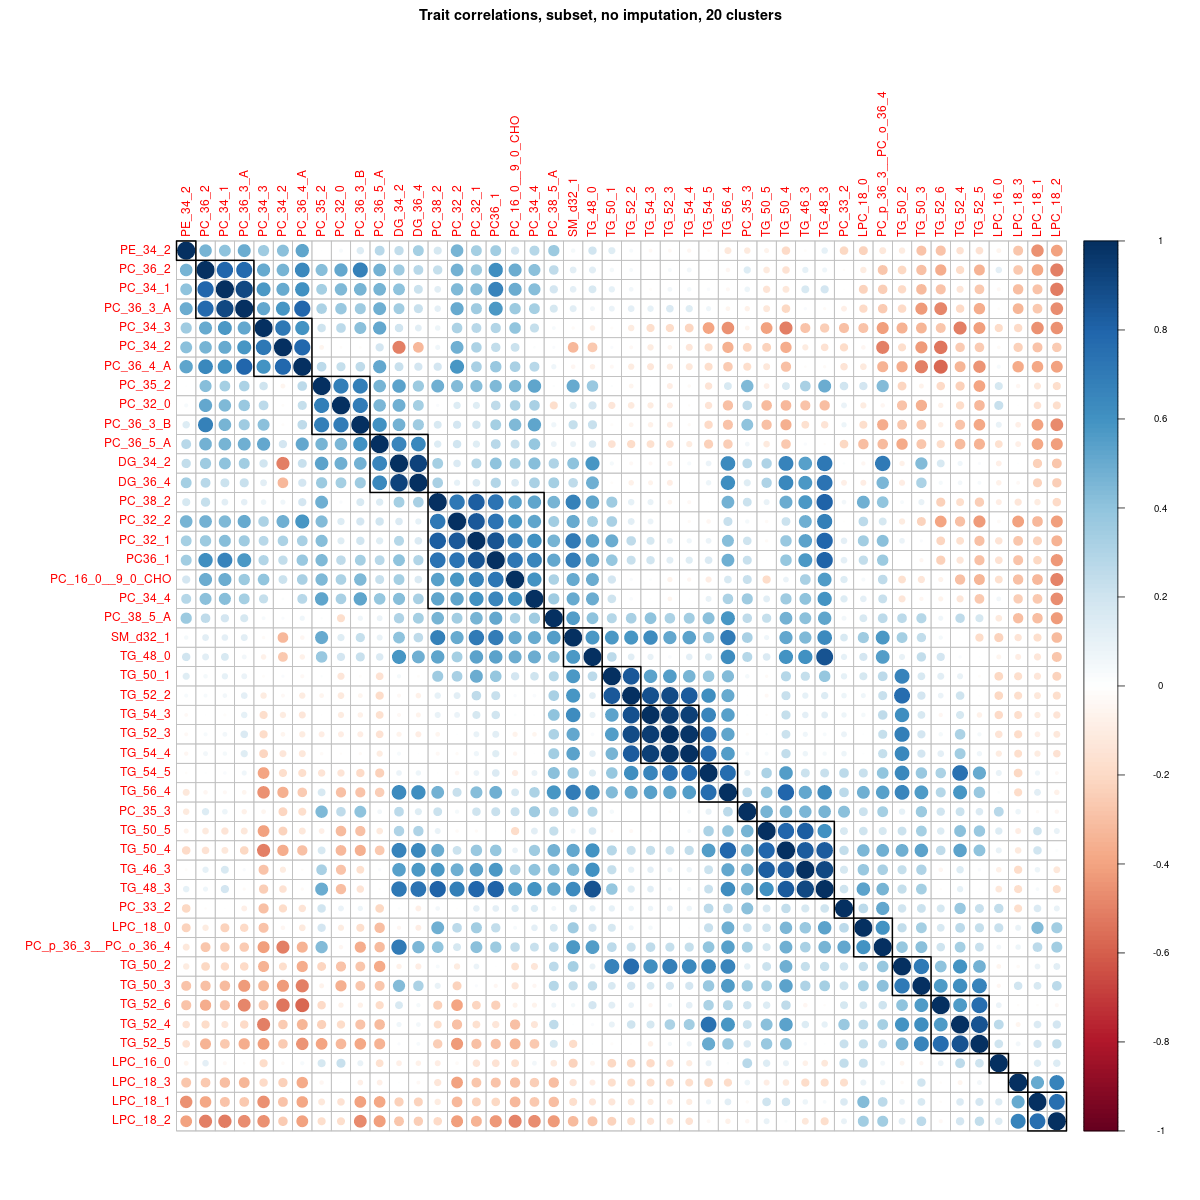
\includegraphics[width=0.9\paperwidth]{Sup_Figures/Sup_Fig_1.png}
\caption{\textit{Pcadapt} analysis of Mexican landraces. We used GBS data from the Mexican landraces of the SeeD dataset \cite{Romero_Navarro2017-cn} and run a \textit{pcadat} analysis \cite{Luu2017-ws} that identified \textbf{A)} elevation as the major driver of population differentiation polarizing PC1.  
\textbf{B)} Genome wide analysis of \textit{Pcadapt} PC1 outliers. 
\textbf{C)} Population Branch Excess Analysis of glycerolipid pathway genes.
From the initial set of 211 genes we used 186 genes with 6219 non redundant SNPs and 683162 non redundant SNPs for the SW US group; 186 genes with 6106 non redundant SNPs and 664555 non redundant SNPs for the Mexican Highland group; 185 genes with 5912 non redundant SNPs and 641186 non redundant SNPs for the Guatemalan Highlands group; and 184 genes with 5698 non redundant SNPs and 614783 non redundant SNPs for the Andes group.
\textbf{D)} Highland selection of Glycerolipid pathways using PBE. See methods for details.
For each pathway, we first selected all SNPs in the CDS regions and 10Kb upstream and downstream of the gene and we calculated the mean pathway PBE score. 
We then constructed a null distribution by drawing 10000 samples without replacement of $n$ SNPs from those found within or around 10Kb upstream and downstream of all protein coding genes and we obtained the mean PBE for this null distribution. 
For each pathway, the heat map shows p-values corresponding to the probability of sampling from the null distribution a set of $n$ SNPs with the observed glycerolipid pathway mean PBE score or higher. 
}
\label{SupFig1}
\end{center}
\end{figure*} 

\clearpage

\begin{figure*}[t]
\begin{center}
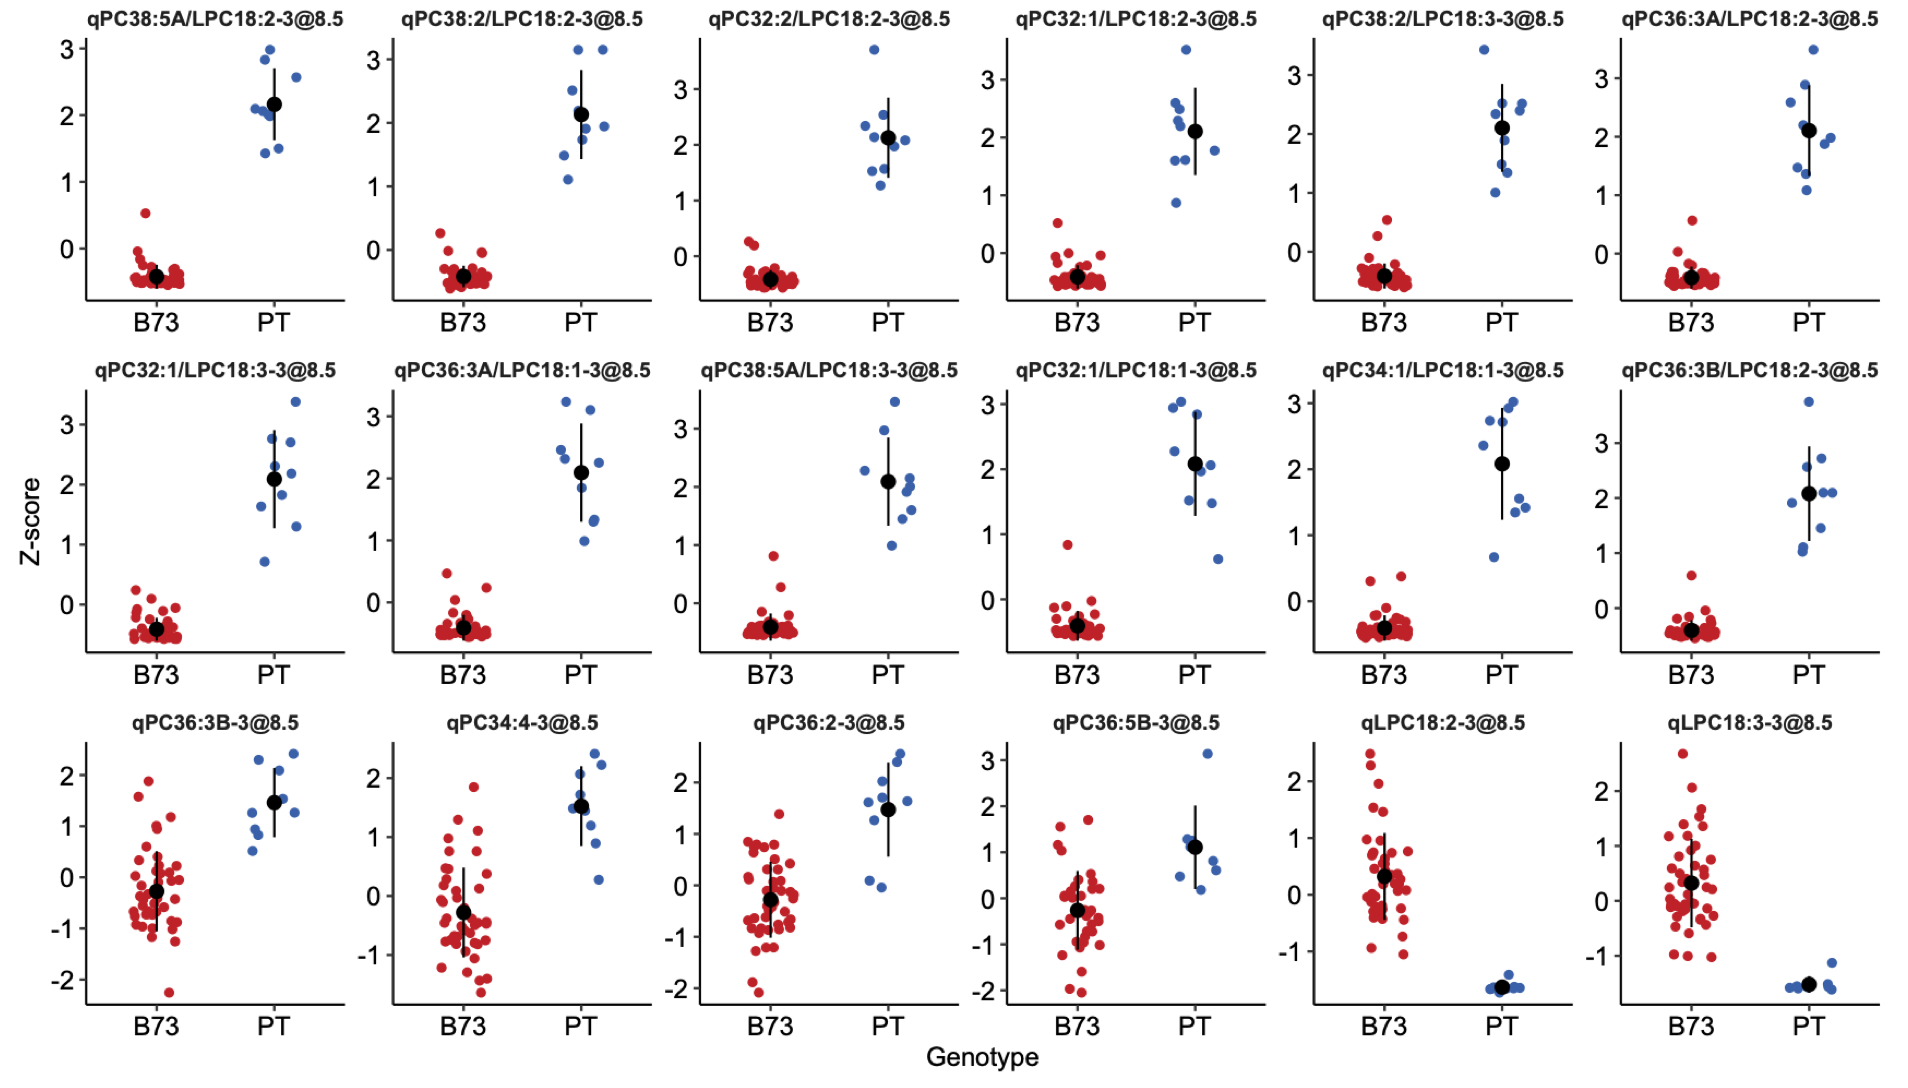
\includegraphics[width=0.9\paperwidth]{Sup_Figures/Sup_Fig_2.png}
\caption{Effects of QTLs at 3@8.5 for individual PC and LPC species (bottom), and PC/LPC ratios (12 most significant peaks).
}

\label{SupFig2}
\end{center}
\end{figure*} 

\clearpage

\begin{figure}[t]
\begin{center}
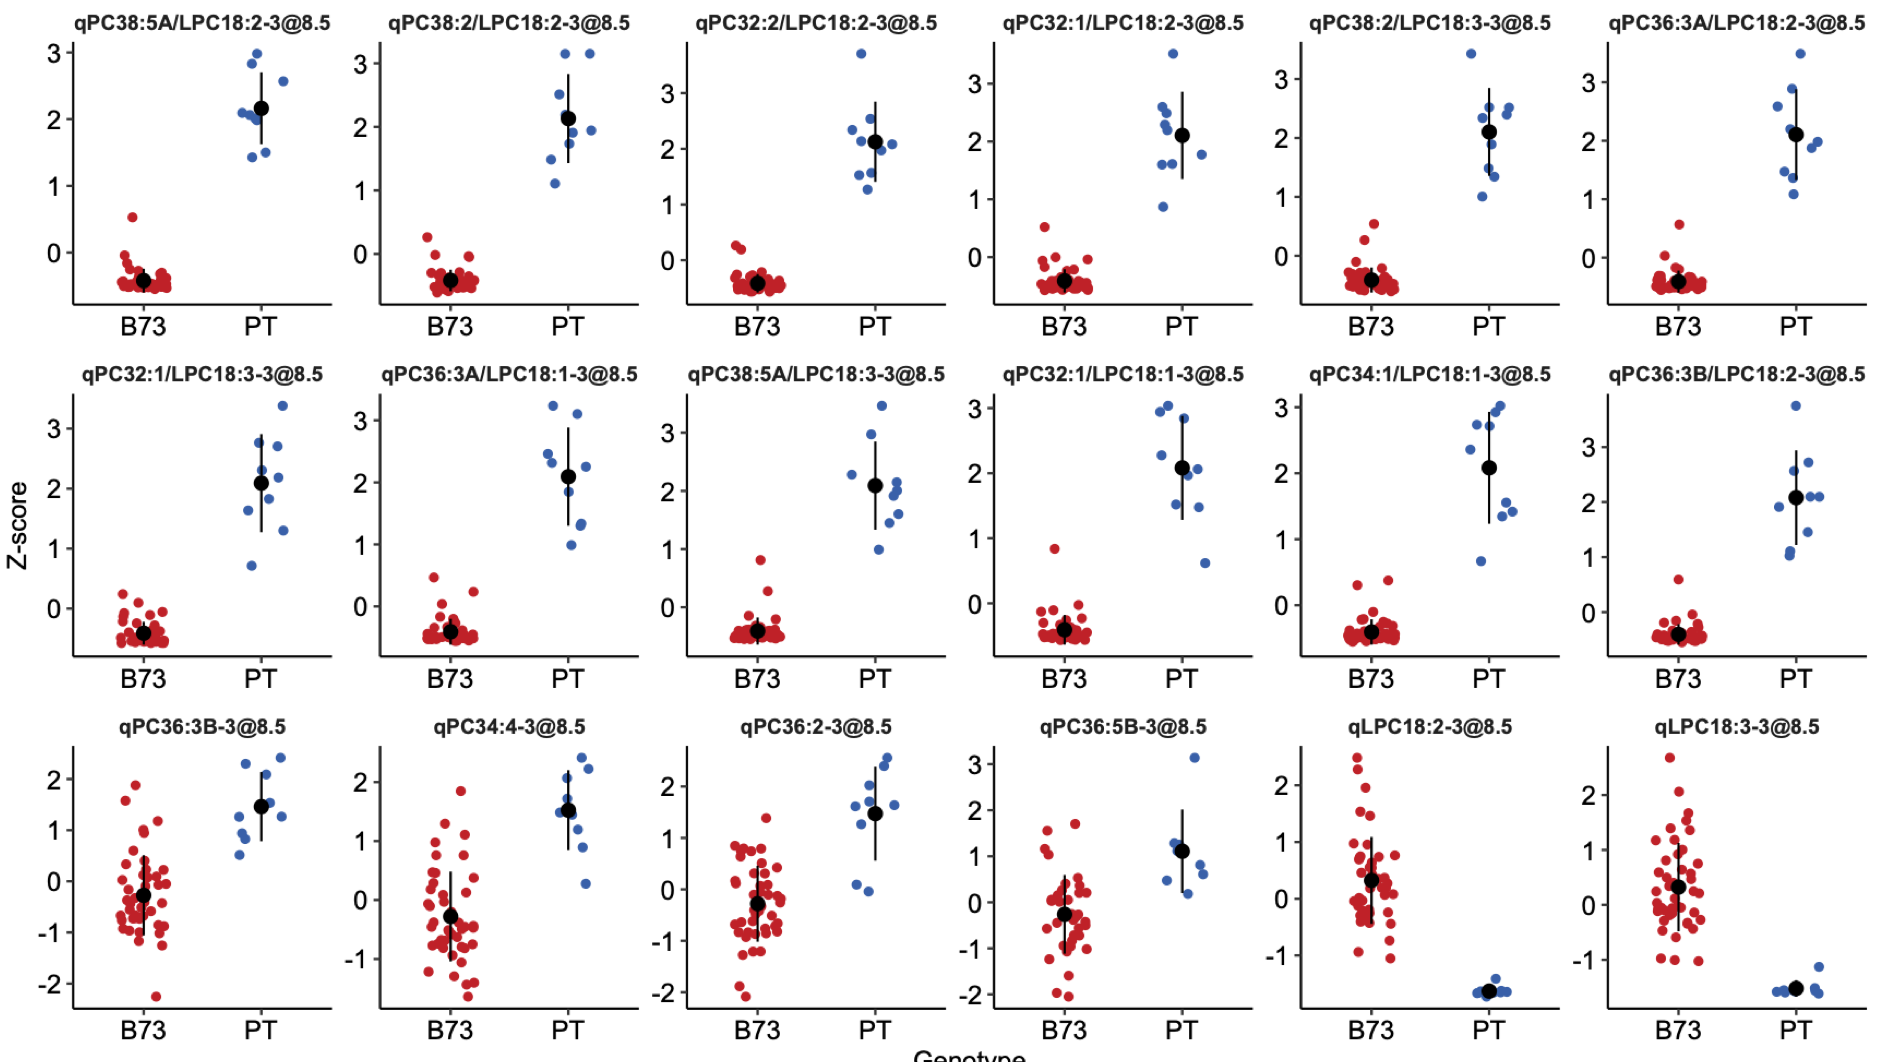
\includegraphics[width=0.4\paperwidth]{Sup_Figures/Sup_Fig_3.png}
\caption{\textbf{A)} Genomic Location of genes coding for enzymes predicted Phospholipase A1 activity. 
\textbf{B)} Site of action of the different types of phospholipases.
\textbf{C)} Effect sizes of PC/LPC levels at RILs homozyzogous B73, PT and heterozygous qPC/LPC3@8.5.
} 
\label{SupFig3}
\end{center}
\end{figure}  


\clearpage

\begin{figure}[t]
\begin{center}
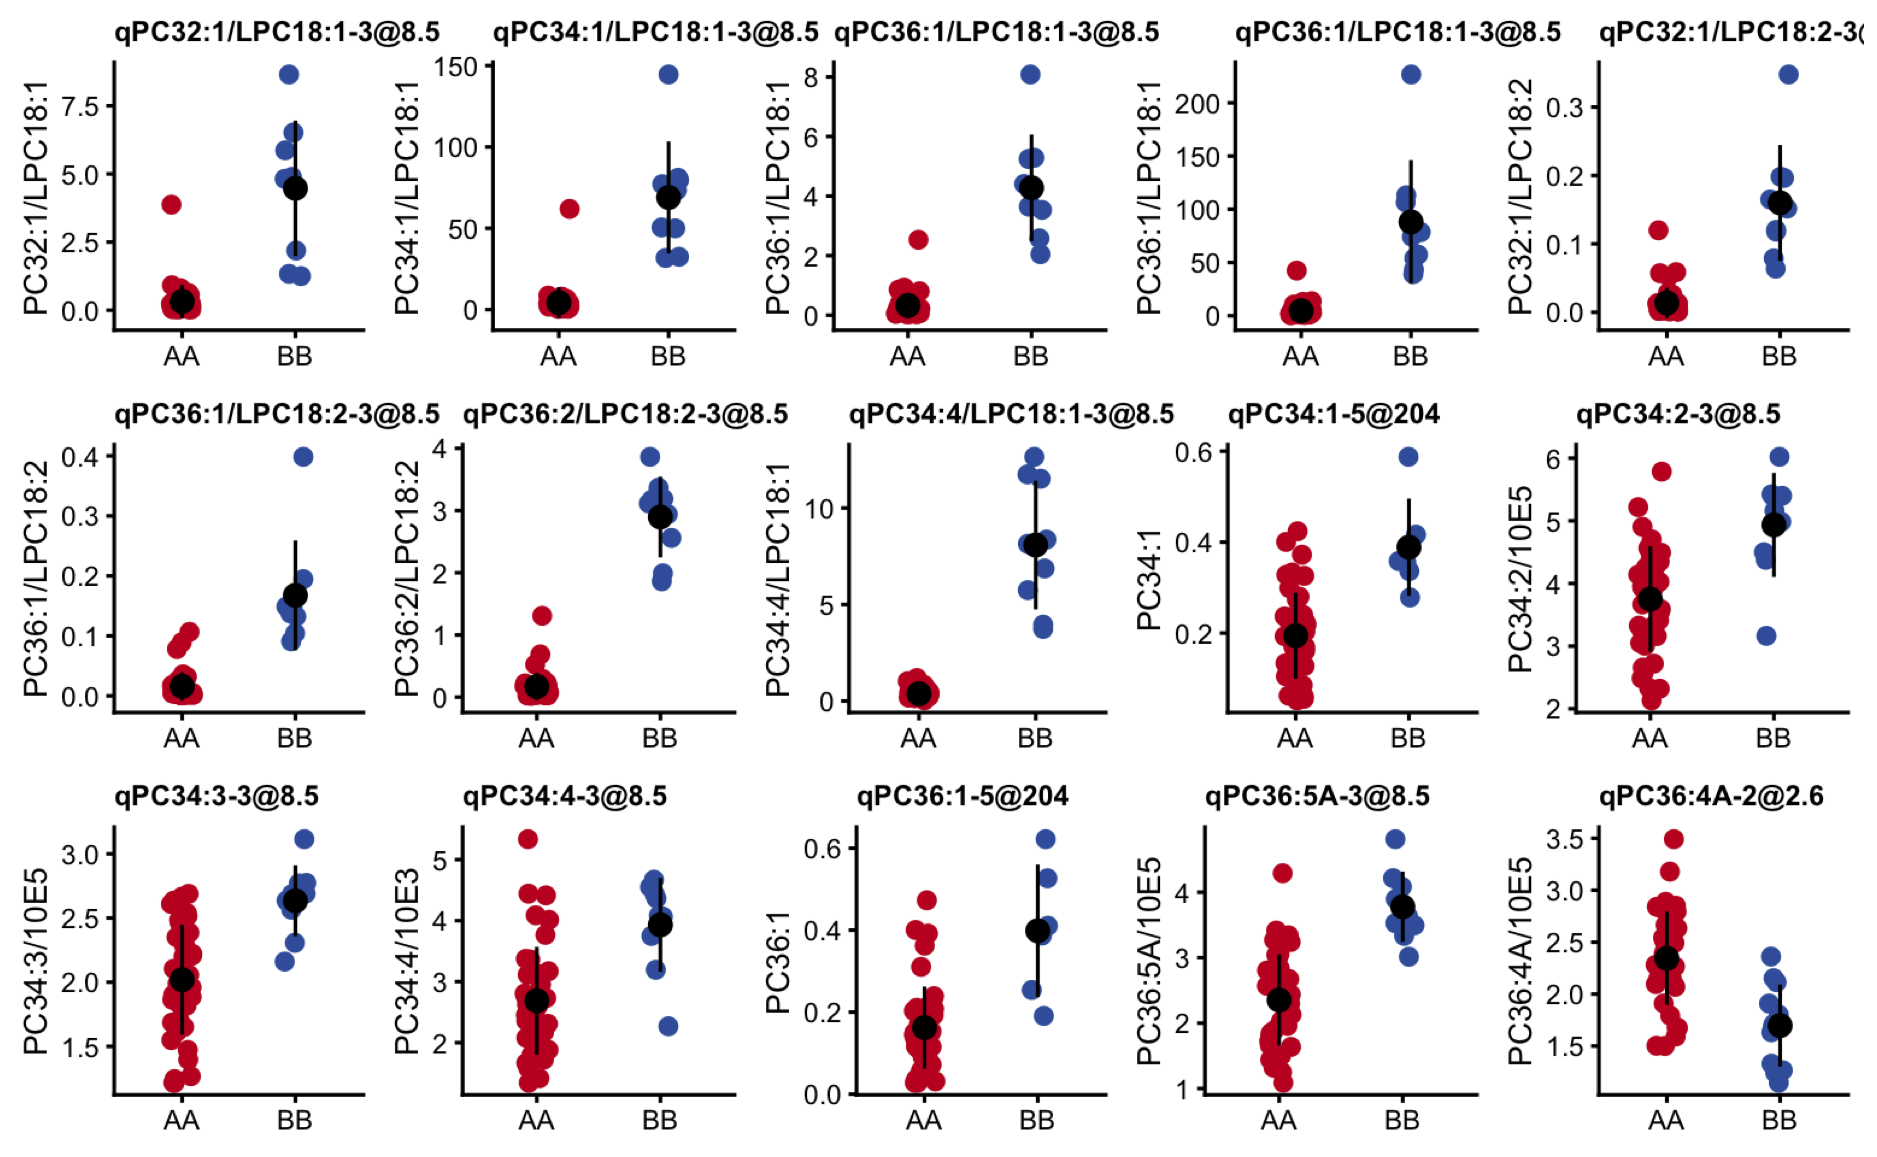
\includegraphics[width=0.6\paperwidth]{Sup_Figures/Sup_Fig_4.png}
\caption{\textbf{Subcellular localization of \textit{HPC1} in \textit{Nicotiana benthamiana} leaf cells.}   
CTP.HPC1-GFP, 52 amino acids of the phospholipase were fused to GFP. 
Three constructs encoding subcellular localization signals were used as control; Cytoplasm (C-GFP), nucleus (N-GFP), and Chloroplast (P-GFP). All of them under control of the 35S promoter. The write arrows show chloroplast and nucleus.
}
\label{SupFig4}
\end{center}
\end{figure} 

\begin{figure}[t]
\begin{center}
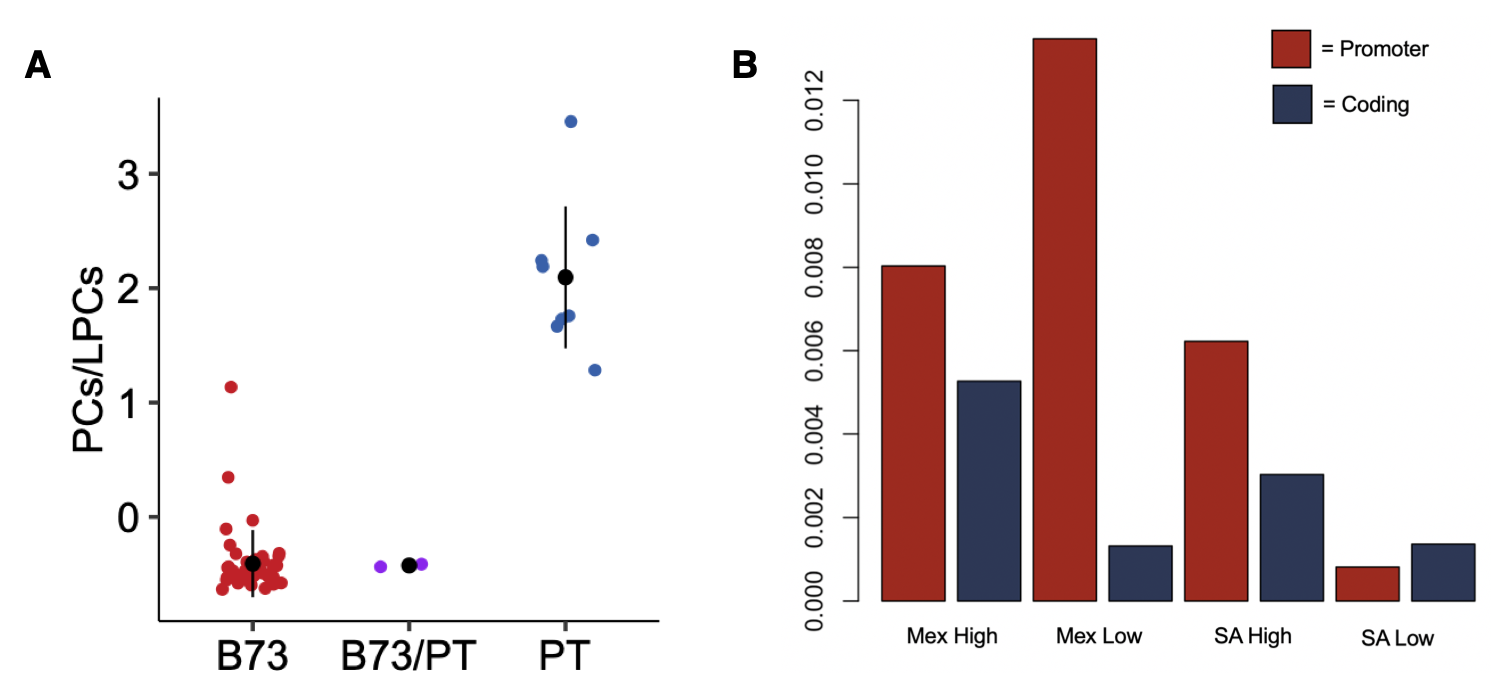
\includegraphics[width=0.8\paperwidth]{Sup_Figures/Sup_Fig_5.png}
\caption{\textbf{A)} B73 expression levels of genes coding for enzymes with predicted Phospholipase A1 activity across different tissues. \textit{HPC1} is indicated in blue. 
Data from \cite{Stelpflug2016-vr}.
\textbf{B)} B73 leaf tissue expression levels of genes in the 7.9 - 10 Mb QTL interval of chr 3. 
Data from \cite{Stelpflug2016-vr}.
\textbf{C)} \textit{HPC1} expression levels of temperate inbred lines B73, Mo17, OH43, and PH207 under control, control and heat stress. Values taken from \cite{Waters2017-nat}
} 
\label{SupFig5}
\end{center}
\end{figure} 

\clearpage

\begin{figure*}[t]
\begin{center}
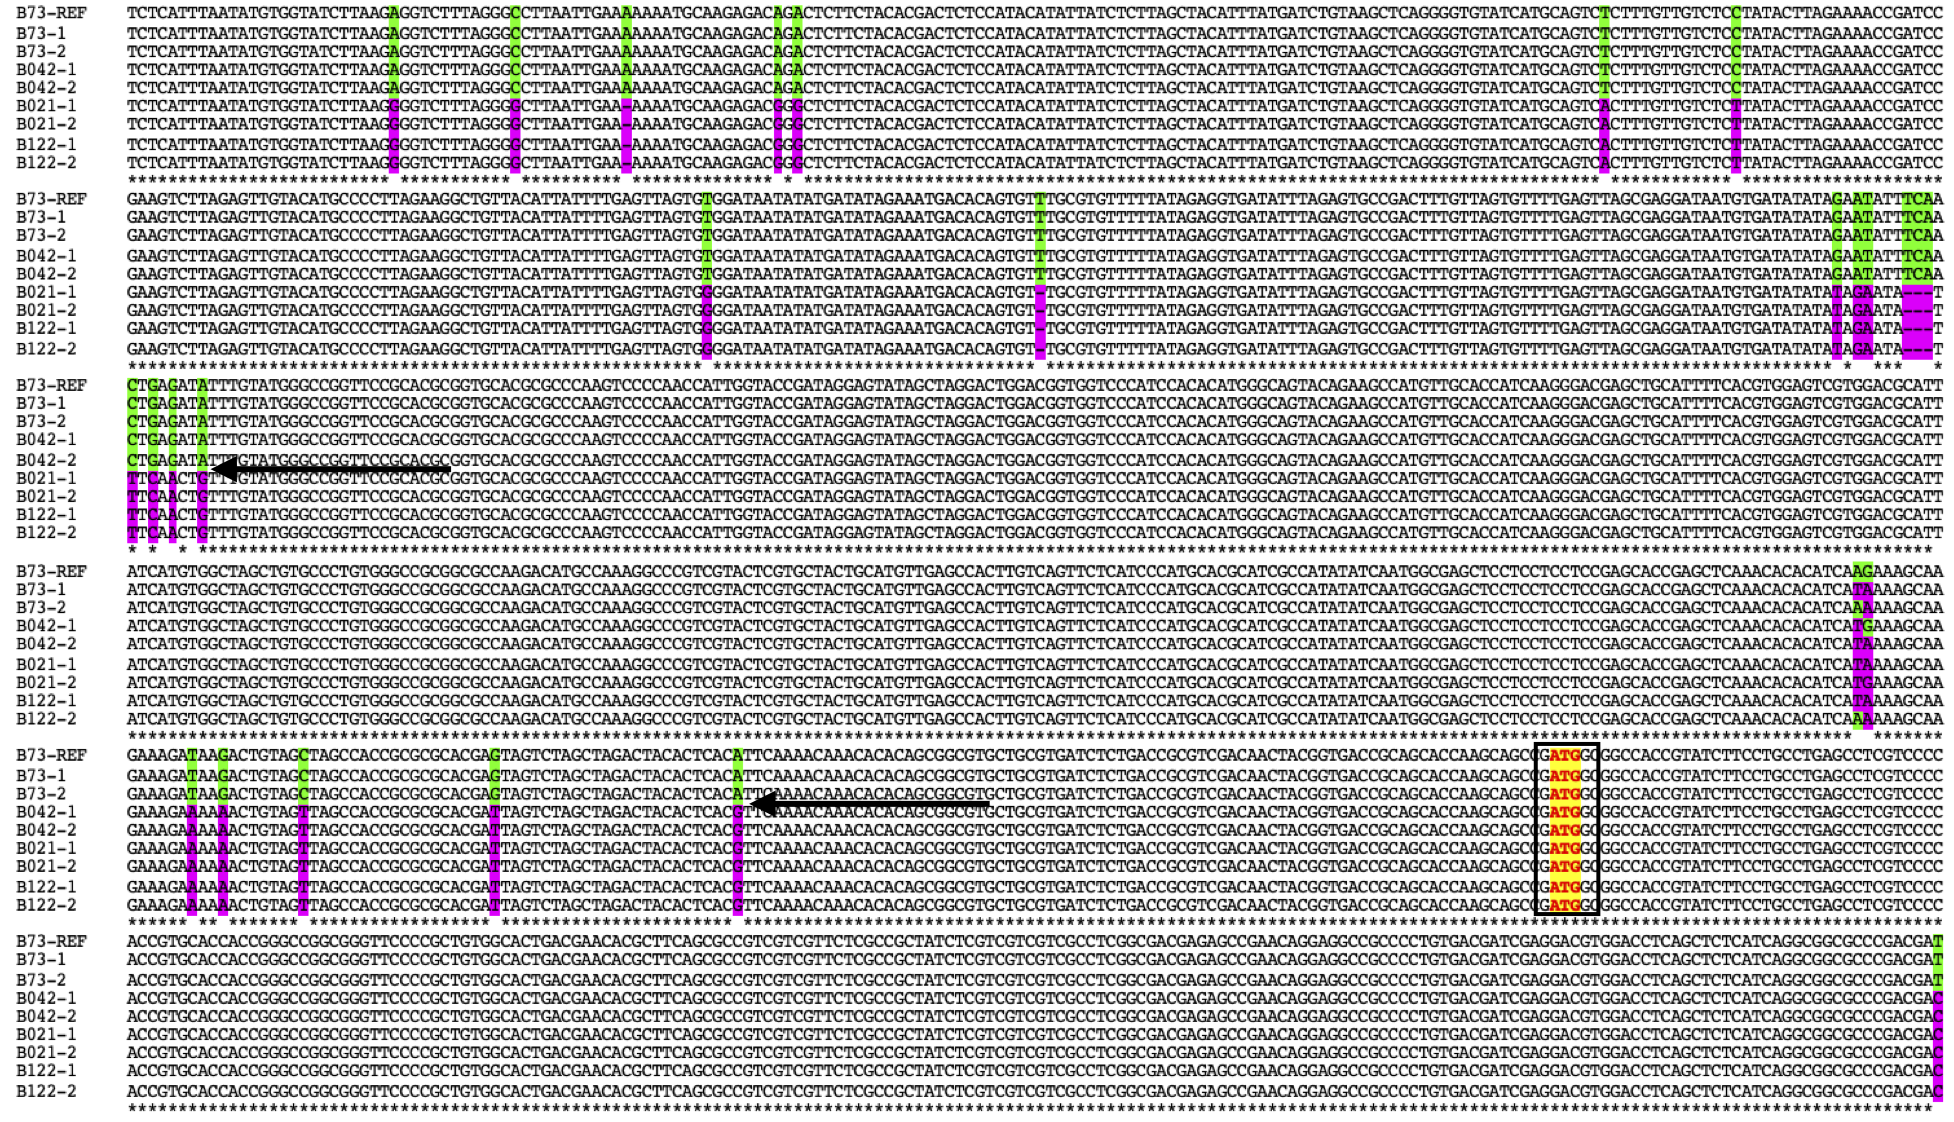
\includegraphics[width=0.9\paperwidth]{Sup_Figures/Sup_Fig_6.png}
\caption{Sanger sequencing of the promoter and start of the \textit{HPC1} sequence obtained from B73 plants and 3 RILs (B042, B021 and B122). A recombination point 500 bp upstream the ATG in B104 is indicated by arrows. B73 alleles are marked in green and PT alleles are marked in pink. 
}
\label{SupFig6}
\end{center}
\end{figure*} 


\clearpage

\begin{figure*}[t]
\begin{center}
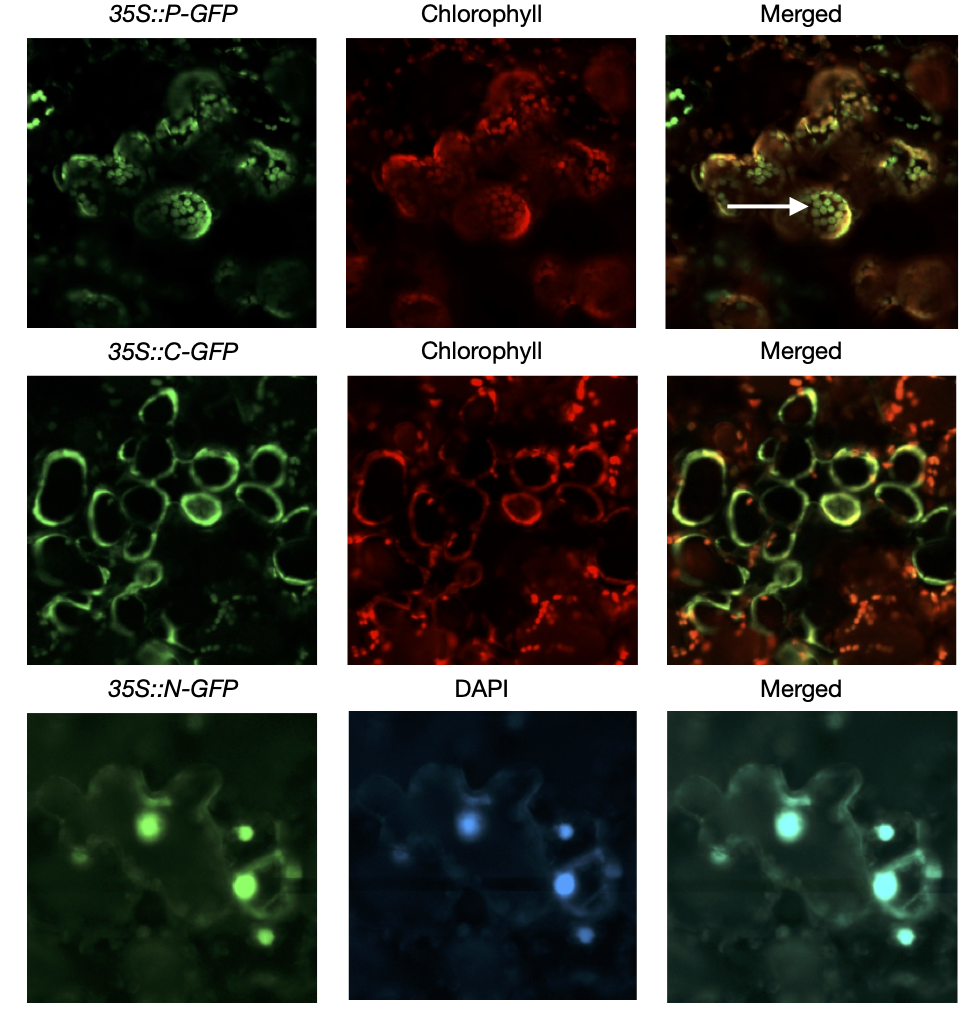
\includegraphics[width=0.6 \paperwidth]{Sup_Figures/Sup_Fig_7.png}
\caption{Flowering time and phospholipid related gene expression correlation with flowering time traits in aerial tissues in the 282 panel. 
Data obtained from \cite{Kremling2018-gn}}.
\label{SupFig7}
\end{center}
\end{figure*} 

\clearpage

%\begin{figure}[t]
%\begin{center}
%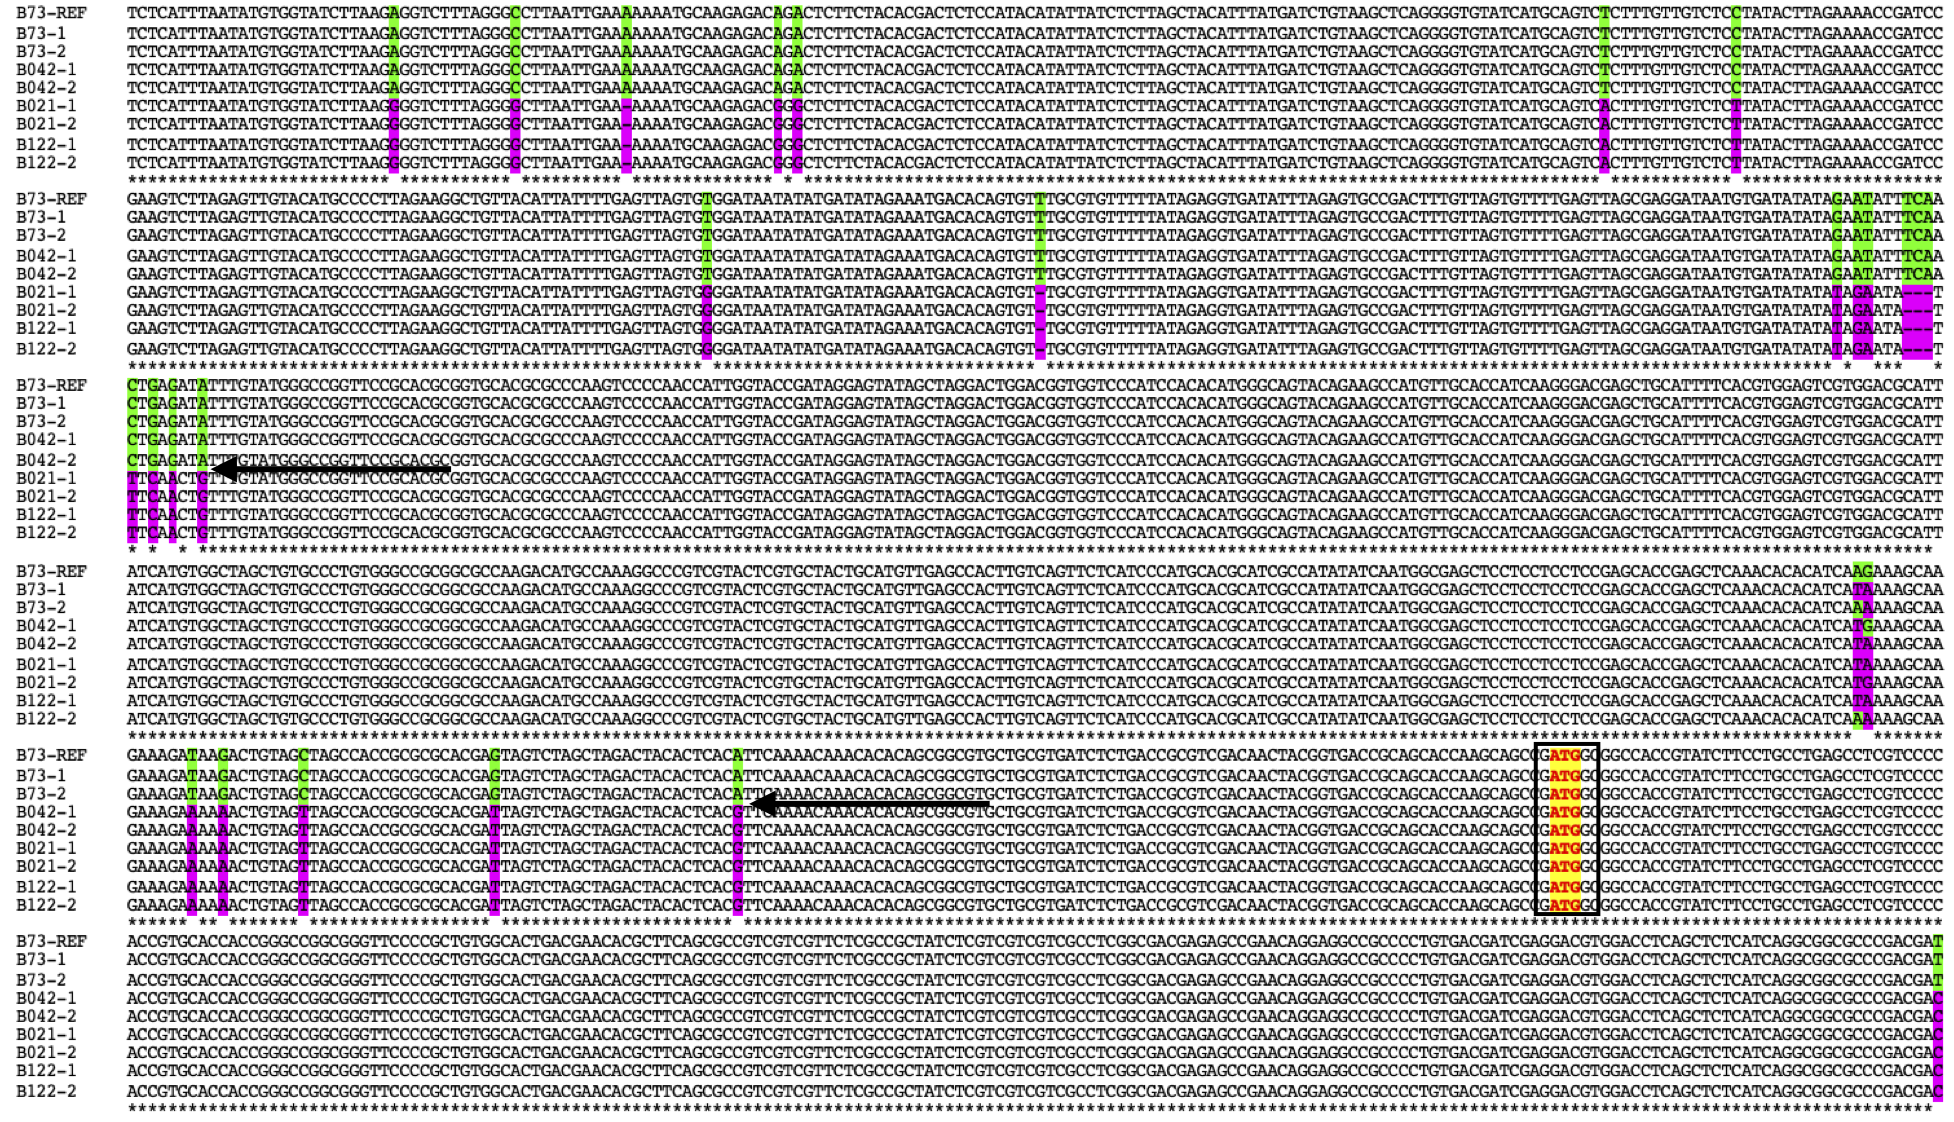
\includegraphics[width=0.6\paperwidth]{Sup_Figures/Sup_Fig_6.png}
%\caption{\textbf{A)} Nucleotidy diversity analysis of the promoter and CDS region of \textit{HPC1} using whole genome %sequencing data of highland and lowland landraces México and South American.
%}
%\label{SupFig6}
%\end{center}
%\end{figure} 

%\clearpage

%\begin{figure*}[t]
%\begin{center}
%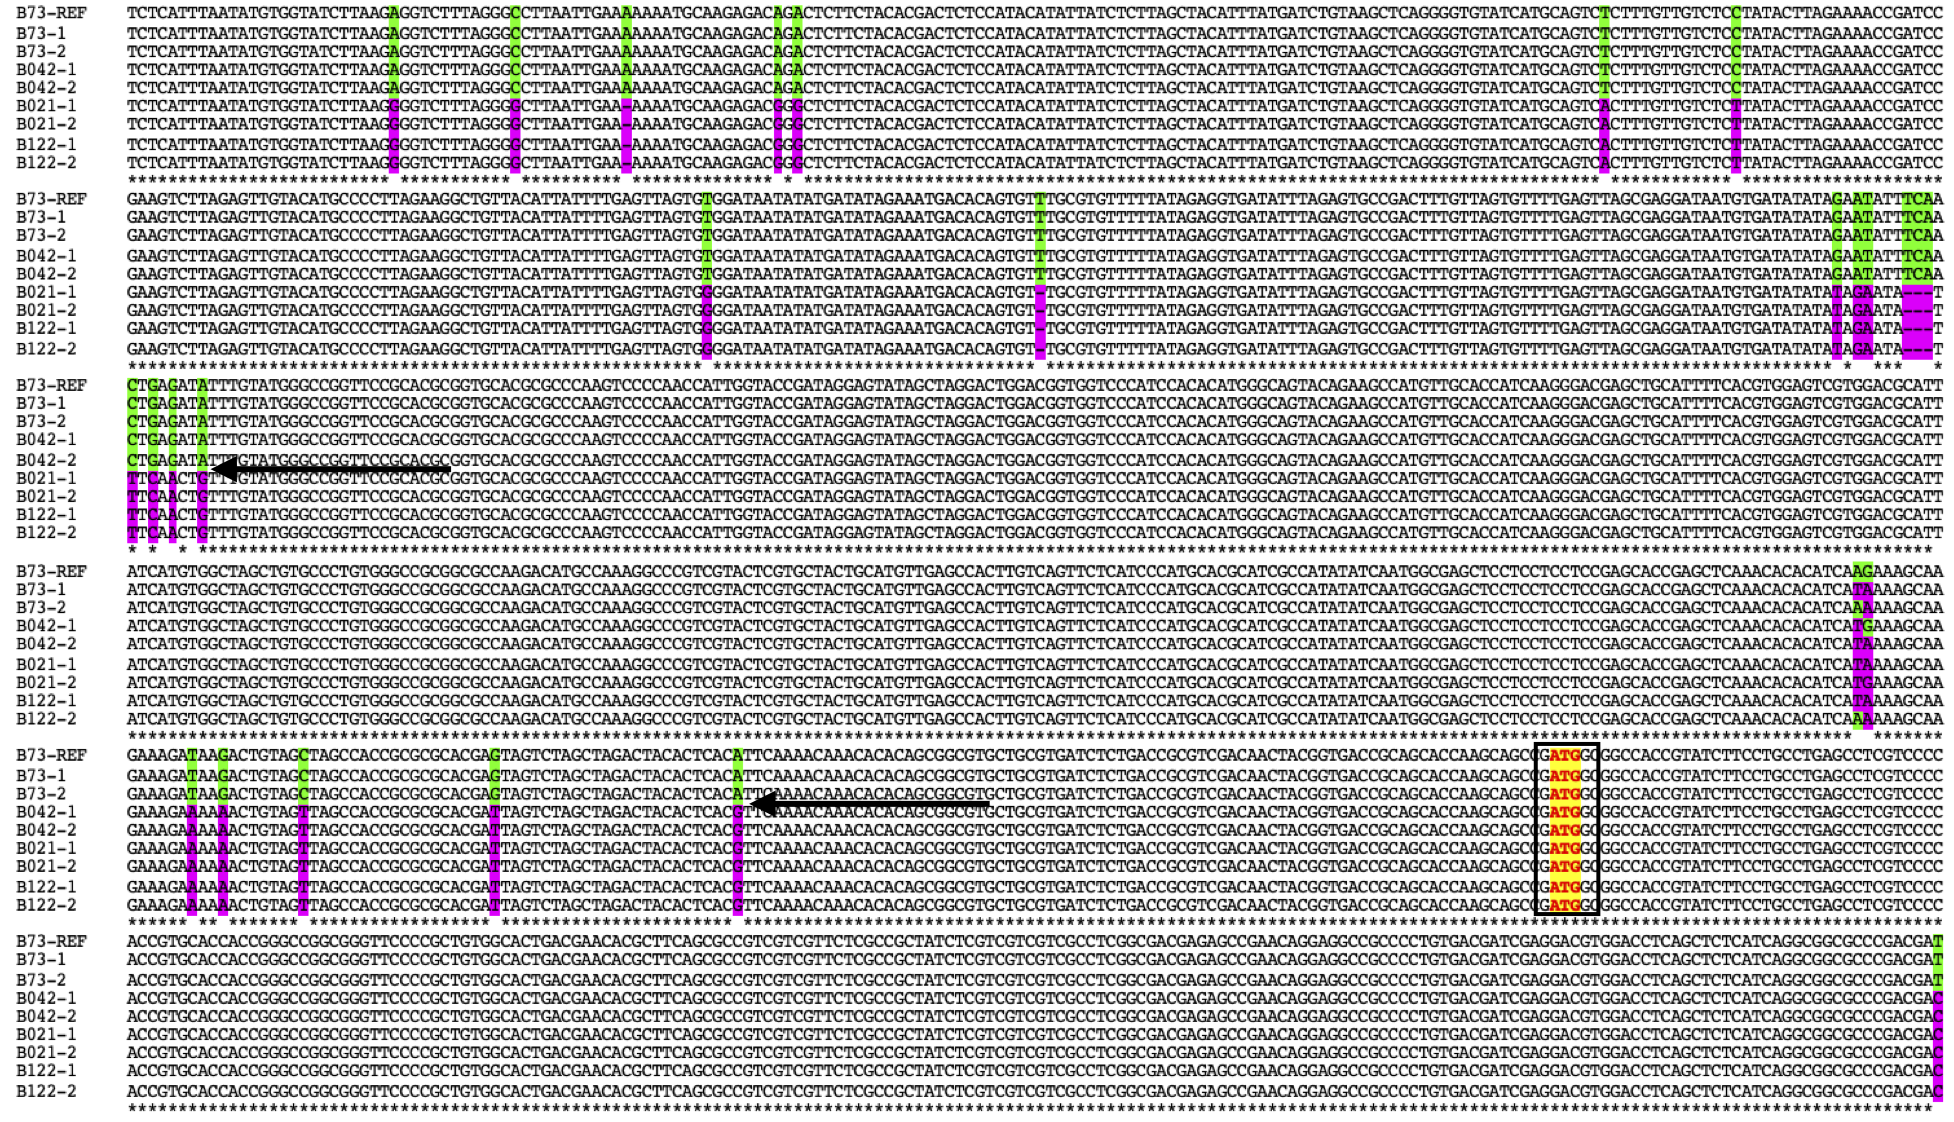
\includegraphics[width=0.8\paperwidth]{Sup_Figures/Sup_Fig_6.png}
%\caption{\textbf{A)} Flag leaf phosphorus levels of B73 and 10 highland landraces each from México and Perú grown in control conditions.
%\textbf{B)} Andosol soil frequency measured using the geographic coordinates of landrace accessions from the SeeD dataset calculated using the soilP package \cite{Rodriguez-Zapata2018-vz}.
%\textbf{C)} Phosphorus content on the \textit{HPC1\textsuperscript{CR}} mutants grown in long day conditions in Clayton, NC.
%\textbf{D)} PCA analysis of ionomics data of the \textit{HPC1\textsuperscript{CR}} mutants and control plants grown in long day conditions in Raleigh.
%}
%\label{SupFig6}
%\end{center}
%\end{figure*} 


\end{document}
